\documentclass[ngerman]{sig-alternate-05-2015}

\usepackage[utf8]{inputenc}
\usepackage[ngerman]{babel}
\usepackage[autostyle=true,german=quotes]{csquotes}
\usepackage{hyperref}
\usepackage{cleveref}
\usepackage{caption}
\usepackage{subcaption}
\usepackage[table]{xcolor}

%%%%%%%%%%%%%%%%
% cheating
%\usepackage{setspace}
%\setstretch{.9865}
%\setstretch{1.1}
%%%%%%%%%%%%%%%%

\makeatletter
\def\@copyrightspace{\relax}
\makeatother

\makeatletter
% don't use hardwired names
\def\fnum@figure{\figurename\ \thefigure}
\def\fnum@table{\tablename\ \thetable}
\patchcmd{\thebibliography}{References}{\refname}{}{}
\patchcmd{\thebibliography}{References}{\refname}{}{}
% fix a silly usage of \uppercase in \@sect
\patchcmd{\@sect}{\uppercase}{\MakeUppercase}{}{}
\patchcmd{\@sect}{\uppercase}{\MakeUppercase}{}{}
\makeatother

\crefformat{footnote}{#2\footnotemark[#1]#3}

\begin{document}

% Copyright
%\setcopyright{acmcopyright}
%\setcopyright{acmlicensed}
%\setcopyright{rightsretained}
%\setcopyright{usgov}
%\setcopyright{usgovmixed}
%\setcopyright{cagov}
%\setcopyright{cagovmixed}


% DOI
%\doi{10.475/123_4}

% ISBN
%\isbn{123-4567-24-567/08/06}

%Conference
%\conferenceinfo{PLDI '13}{June 16--19, 2013, Seattle, WA, USA}

%\acmPrice{\$15.00}

%
% --- Author Metadata here ---
%\conferenceinfo{WOODSTOCK}{'97 El Paso, Texas USA}
%\CopyrightYear{2007} % Allows default copyright year (20XX) to be over-ridden - IF NEED BE.
%\crdata{0-12345-67-8/90/01}  % Allows default copyright data (0-89791-88-6/97/05) to be over-ridden - IF NEED BE.
% --- End of Author Metadata ---

\title{SecureBlue++: CPU Support for Secure Executables}
%\subtitle{[Extended Abstract]
%\titlenote{A full version of this paper is available as
%\textit{Author's Guide to Preparing ACM SIG Proceedings Using
%\LaTeX$2_\epsilon$\ and BibTeX} at
%\texttt{www.acm.org/eaddress.htm}}}
%
% You need the command \numberofauthors to handle the 'placement
% and alignment' of the authors beneath the title.
%
% For aesthetic reasons, we recommend 'three authors at a time'
% i.e. three 'name/affiliation blocks' be placed beneath the title.
%
% NOTE: You are NOT restricted in how many 'rows' of
% "name/affiliations" may appear. We just ask that you restrict
% the number of 'columns' to three.
%
% Because of the available 'opening page real-estate'
% we ask you to refrain from putting more than six authors
% (two rows with three columns) beneath the article title.
% More than six makes the first-page appear very cluttered indeed.
%
% Use the \alignauthor commands to handle the names
% and affiliations for an 'aesthetic maximum' of six authors.
% Add names, affiliations, addresses for
% the seventh etc. author(s) as the argument for the
% \additionalauthors command.
% These 'additional authors' will be output/set for you
% without further effort on your part as the last section in
% the body of your article BEFORE References or any Appendices.

\numberofauthors{2} %  in this sample file, there are a *total*
% of EIGHT authors. SIX appear on the 'first-page' (for formatting
% reasons) and the remaining two appear in the \additionalauthors section.
%
\author{
% You can go ahead and credit any number of authors here,
% e.g. one 'row of three' or two rows (consisting of one row of three
% and a second row of one, two or three).
%
% The command \alignauthor (no curly braces needed) should
% precede each author name, affiliation/snail-mail address and
% e-mail address. Additionally, tag each line of
% affiliation/address with \affaddr, and tag the
% e-mail address with \email.
%
% 1st. author
\alignauthor
Stephan Mielke\\
       \affaddr{Institut für Programmierung und Reaktive Systeme}\\
       \affaddr{Mühlenpfordtstraße 23}\\
       \affaddr{Braunschweig, Deutschland}\\
       \email{s.mielke@tu-bs.de}
\alignauthor
Nico Weichbrodt\\
	\affaddr{Institut für Betriebssysteme und Rechnerverbund}\\
	\affaddr{Mühlenpfordtstraße 23}\\
	\affaddr{Braunschweig, Deutschland}\\
	\email{weichbr@ibr.cs.tu-bs.de}
}
% There's nothing stopping you putting the seventh, eighth, etc.
% author on the opening page (as the 'third row') but we ask,
% for aesthetic reasons that you place these 'additional authors'
% in the \additional authors block, viz.
%\additionalauthors{Additional authors: John Smith (The Th{\o}rv{\"a}ld Group,
%email: {\texttt{jsmith@affiliation.org}}) and Julius P.~Kumquat
%(The Kumquat Consortium, email: {\texttt{jpkumquat@consortium.net}}).}
\date{21 Dezember 2016}
% Just remember to make sure that the TOTAL number of authors
% is the number that will appear on the first page PLUS the
% number that will appear in the \additionalauthors section.

\maketitle
\begin{abstract}
SecureBlue++ ist eine seit 2011 von IBM in Entwicklung befindliche CPU-Befehlssatzerweiterung zum verschlüsselten Verteilung, Speichern und Ausführen von Applikationen auf der POWER Architektur \cite{boiviesecureblue++:small,boivie2013secureblue++:big,ibm:homelandsecurity,secureblue++patent}.  Durch diese Abschottung ist es möglich den Angriffsvektor auf die eigene Software ohne große Änderungen zu reduzieren. Jedoch ergeben sich durch den Einsatz von SecureBlue++ nicht nur Vorteile, sondern auch Nachteile in Form von Leistungseinbußen und gravierenden Einschränkungen, welche eine Nutzung im gängigen Cloud-Computing-Szenario nahezu unmöglich machen. 
\end{abstract}

%\keywords{ACM proceedings; \LaTeX; text tagging}

\section{Motivation}
\label{sec:bedrohungsszenario} 
Das Thema Cloud-Computing ist seit einigen Jahren immer mehr ein Thema und viele Unternehmen wollen nicht mehr eigene teure Rechenzentren betreiben, sondern nur noch Rechenzeit bei den sogenannten Cloud-Anbietern, wie zum Beispiel Amazon, Microsoft oder Google kaufen. Jedoch können diese Anbieter wegen dem amerikanischen Recht nicht garantieren, das ihre Server immer wie vom Kunden gewünscht die Anwendungen Ausführen, oder ob sie zusätzlich die Daten der Anwendungen an Dritte weiter geben müssen \cite{poplak2013edward}. Jedoch sind nicht nur staatliche Anordnungen eine Gefahr für die Anwendungen der Kunden, sondern ebenfalls infizierte Systeme oder nicht professionelle Administratoren im Cloud-Rechenzentrum. 

Für diese Bedrohungen werden seit einiger Zeit Lösungen, wie zum Beispiel SecureBlue++, entwickelt \cite{evtyushkin2014iso}. Jedoch gibt es noch weitere Bedrohungen aber auf diese versucht SecureBlue++ keine Lösung zu finden. Diese wären:
\begin{itemize}
	\item Programmierfehler und Sicherheitslücken in den Anwendungen
	\item Denial-of-Service Attacken in jeder Form
\end{itemize}

\section{Einleitung}
In dieser Arbeit soll die Befehlssatzerweiterung SecureBlue++ aus dem Paper \cite{boivie2013secureblue++:big} vorgestellt werden. Hierfür wird zuerst erklärt was SecureBlue++ ist und im Anschluss die einzelnen Neuerungen erklärt. Hierfür werden in \cref{sec:instruktionen} die neuen Instruktionen und in \cref{sec:register} die neuen Register vorgestellt. System Calls sind für die gesicherte Ausführung einer Anwendung sehr problematisch, da die Anwendung den Kontrollfluss dem Kernel übergibt und hierbei, Geheimnisse der Anwendung verraten werden können. In \cref{sec:sesc} wird deswegen die Umsetzung mit System Calls behandelt. Für moderne Anwendungen muss die SecureBlue++ Multi-threading unterstützen. Dies wird in \cref{sec:multithreading} behandelt. Wie SecureBlue++ mit virtuellen Maschinen umgeht findet sich in \cref{sec:vms}. Im Anschluss werden Simulationen von SecureBlue++ getestet und aufgezeigt wie viel Leistungseinbußen auftreten können. Zum Abschluss folgt ein Vergleich von SecureBlue++ mit der Konkurrenztechnologie von Intel

\begin{figure}
	\centering
	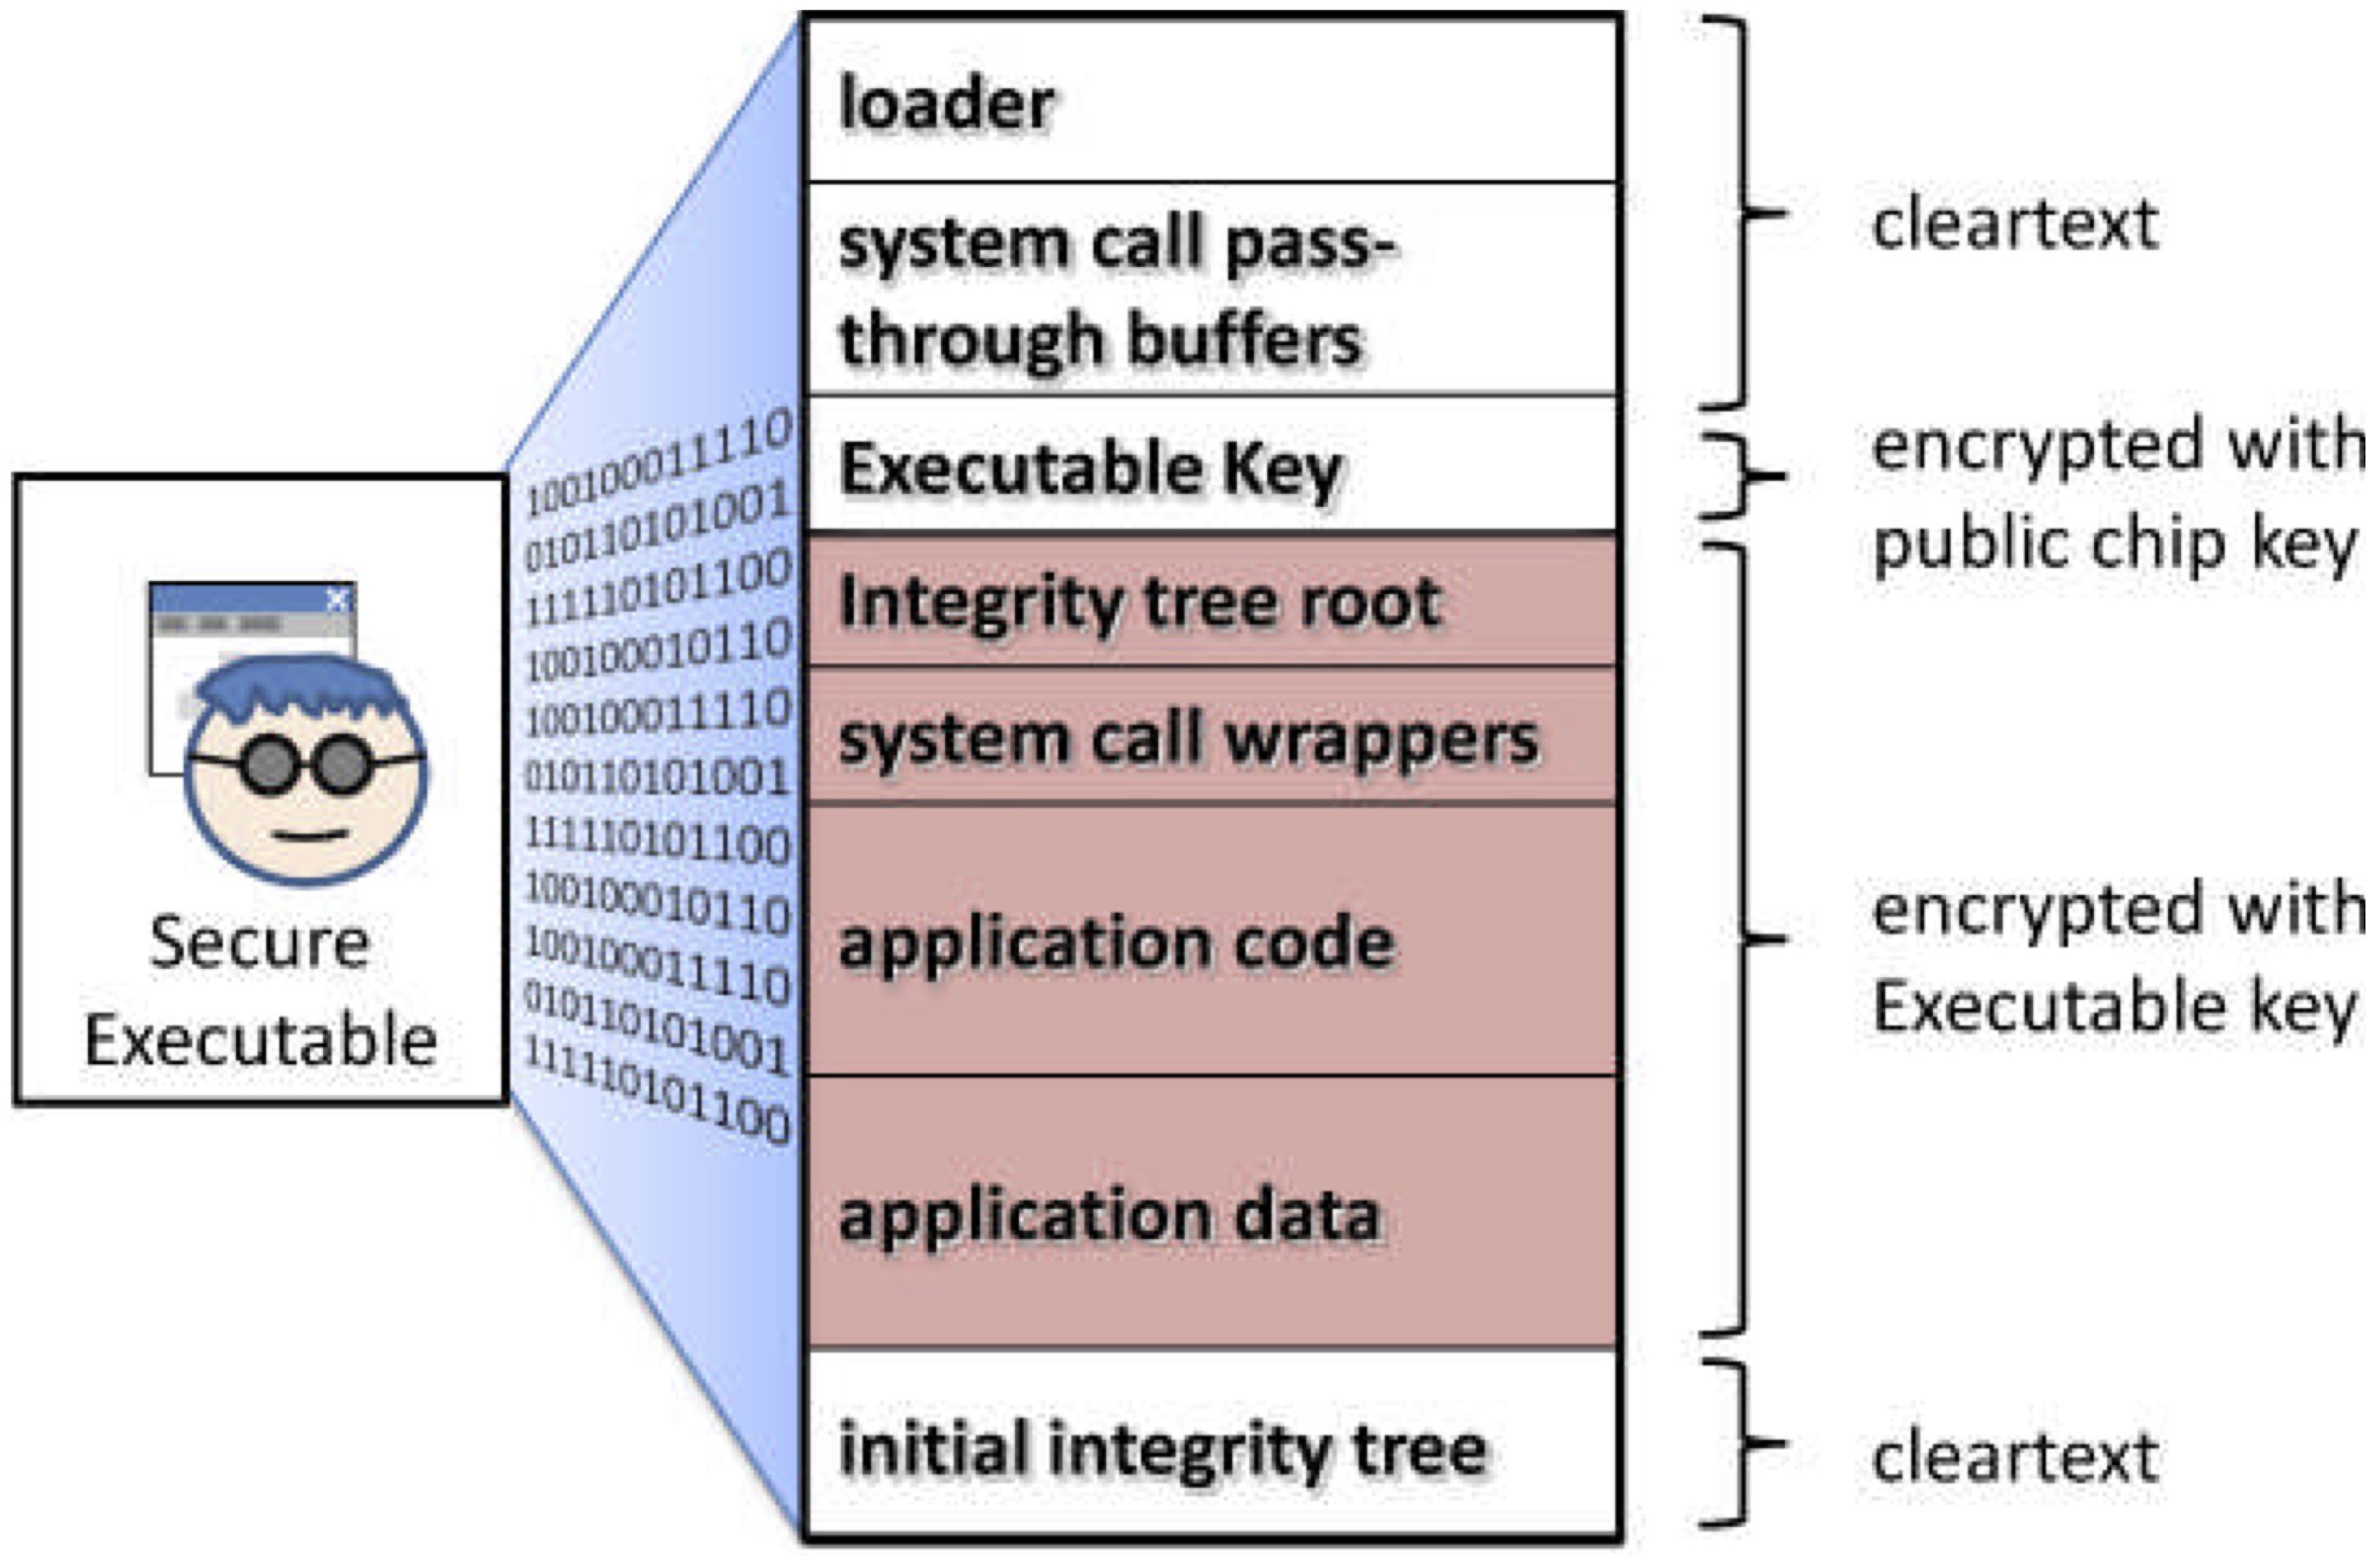
\includegraphics[width=\columnwidth]{aufbau2}
	\caption{Aufbau von mit SecureBlue++ gesicherten ELF Binärdateien. \cite{boivie2013secureblue++:big}}
	\label{fig:aufbau}
\end{figure}

\section{SecureBlue++}
IBM hat seit 2011 die SecureBlue++ CPU-Befehlssatz\-erweiterung in Entwicklung, welche auf der SecureBlue Technologie für Verschlüsselung mit Hardwareunterstützung basiert \cite{ibm_2006, boiviesecureblue++:small}. Mittels dieser Erweiterung können Programme komplett isoliert von anderen Applikationen sowie dem privilegierten Betriebssystem ausgeführt werden. Hierfür wurden neue CPU-Instruktionen und mehrere neue Register eingeführt \cite{boivie2013secureblue++:big}. Des weiteren ist der von der jeweiligen Anwendung belegten Arbeitsspeicher in die Bereiche \enquote{read-only and execute} und \enquote{no-execute} disjunkt geteilt. 

Ein weiteres Feature von SecureBlue++ ist die Möglichkeit eine Applikation verschlüsselt und geschützt durch einen Integritätsbaum auf der Festplatte vorzuhalten, um das Reverse Engineering oder das Manipulieren der Software zu verhindern. Hierfür besitzt jede CPU ein bei der Herstellung festgelegtes Public/Private Key-Paar, von dem der Public Key in einem \enquote{read-only} Register zur Verfügung gestellt wird.

\subsection{Aufbau von gesicherten Anwendungen}
Das Executable and Linking Format ELF Dateiformat ist ein im UNIX Umfeld weit verbreitetes Format für Anwendungen. SecureBlue++ ist konzipiert das es sich bei der Kompilierung von Anwendungen zu ELF Dateien in den beim Linken integriert. Hierdurch wird sichergestellt das keine Änderungen am Quellcode der Anwendung benötigt werden. 
In \cref{fig:aufbau} wird der Aufbau einer mit SecureBlue++ gesicherten Anwendung aufgezeigt. 

Der Loader besteht aus dem in \cref{fig:esm} gezeigten unverschlüsselten Aufruf der \texttt{esm}-Instruktion (\cref{sec:esm}) mit dem öffentlichen Schlüssel verschlüsselte AES-Schlüssel der Anwendung sowie aus den in \cref{sec:metadata} gezeigten Metadaten. Des weiteren werden Buffer für die System Call Wrapper im unverschlüsseltem Speicherbereich bereitgestellt.

Im Anschluss folgen mit dem AES-Schlüssel verschlüsselt die Daten der Anwendung wie dem Integrity Tree (\cref{sec:Integritätsbaum}), den System Call Wrappern (\cref{sec:sesc}) und dem auszuführenden Code sowie den Daten der Anwendung. Am Ende befindet sich ein Hash-Wert zum validieren der ELF Datei.

\subsection{Umsetzung per Hardware}
Für Umsetzung von SecureBlue++ wurde hardwareseitig das Verhalten der POWER CPUs modifiziert.

\begin{figure}
	\centering
	\includegraphics[width=\columnwidth]{ram2}
	\caption{Grundidee: sensible Daten sind innerhalb der CPU unverschlüsselt und nur außerhalb verschlüsselt. \cite{boivie2013secureblue++:big}}
	\label{fig:ram}
\end{figure}
\paragraph{RAM-Verschlüsselung} In \cref{fig:ram} wird die RAM-Verschlüsselung aufgezeigt, bei dem innerhalb der CPU die Daten unverschlüsselt sind und sobald diese die CPU verlassen verschlüsselt werden \cite{secureblue++patent}. Dies wird völlig transparent für die Anwendung und nahezu transparent für das jeweilige Betriebssystem ausgeführt \cite{boivie2013secureblue++:big}. Für die Verschlüsselung kommt ein für die Anwendung eigens generierter AES-Schlüssel zum Einsatz. 

\paragraph{Cache-Line-Verifikation} Mittels des Integritätsbaums werden die Daten beim Laden in die CPU auf ihre Richtigkeit überprüft. Hierbei kann es allerdings zu Leistungseinbußen kommen, wenn die benötigen Teile des Baums nicht im Cache der CPU vorhanden sind und deswegen ebenfalls geladen werden müssen. Beim zurückschreiben von Cache Lines in den RAM wird der Baum dementsprechend automatisch aktualisiert \cite{boivie2013secureblue++:big}. Weitere Informationen folgen in \cref{sec:Integritätsbaum}.

\paragraph{Cache Line-Schutz} Um das Auslesen von Cache Lines zu verhindern, wird jeder Cache Line, einer gesicherten Region, ein Label (\emph{Memory Region ID} \emph{MRID} welche mit der \emph{Secure Executable ID} \emph{SEID} verbunden ist), der dazugehörigen Anwendung, zugeordnet. Wenn eine Anwendung auf eine Cache Line zugreifen will, die mit einem Label versehen ist, werden die \emph{MRID} Werte vergleichen und bei Ungleichheit wird der Zugriff als ein Cache Miss behandelt \cite{boivie2013secureblue++:big}.

\paragraph{Register-Schutz} So lange sich die CPU im Secure-Modus befindet, ändert sie ihr normales Verhalten bei einem Interrupt. Bei jedem Interrupt außer dem (\texttt{sesc}) werden hardwareseitig alle Register mit der jeweiligen \emph{SEID} in der \emph{Thread Restore List} (\emph{TRL}) gespeichert und anschließend mit Nullen überschrieben bevor der Kontrollfluss an den jeweiligen Interrupt Handler des Systems übergeben wird. 

\subsection{Neue Register}
\begin{figure}
	\centering
	\begin{subfigure}[b]{0.26\columnwidth}
		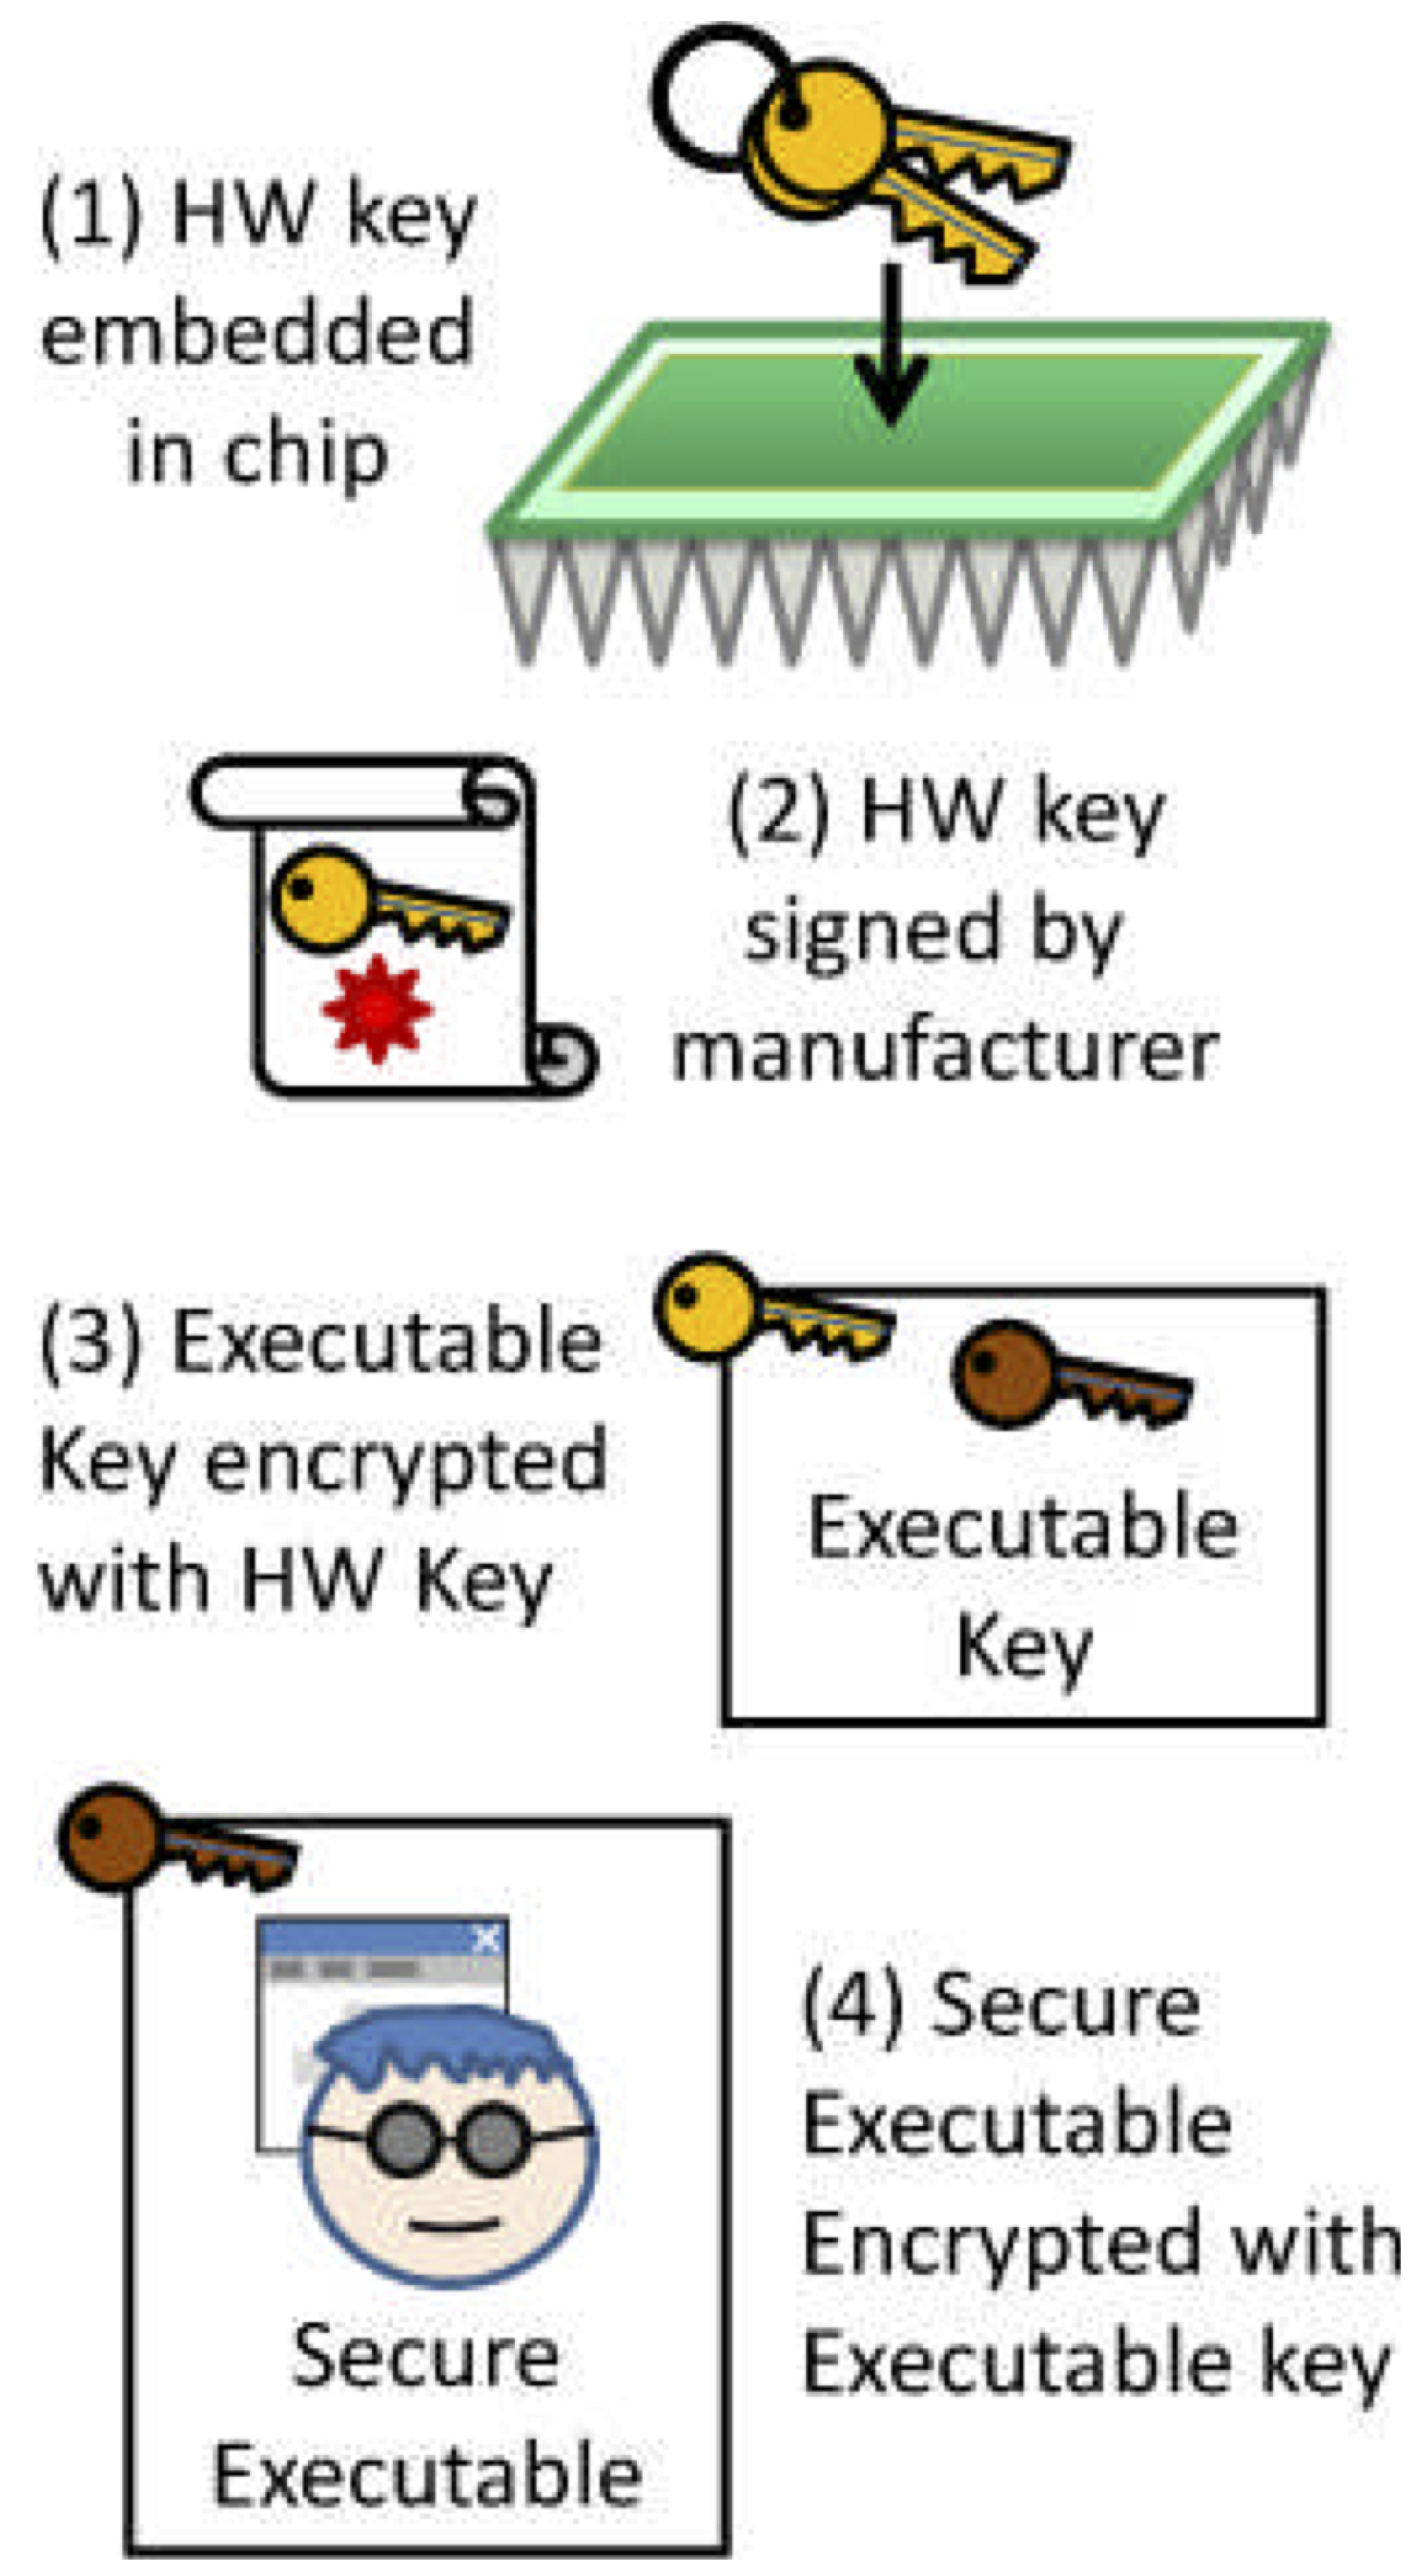
\includegraphics[width=\columnwidth]{hw_key2}
		\caption{Ablauf der Verschlüsselung}
		\label{fig:keys}
	\end{subfigure}
\hfill
	~ %add desired spacing between images, e. g. ~, \quad, \qquad, \hfill etc. 
	%(or a blank line to force the subfigure onto a new line)
	\begin{subfigure}[b]{0.69\columnwidth}
		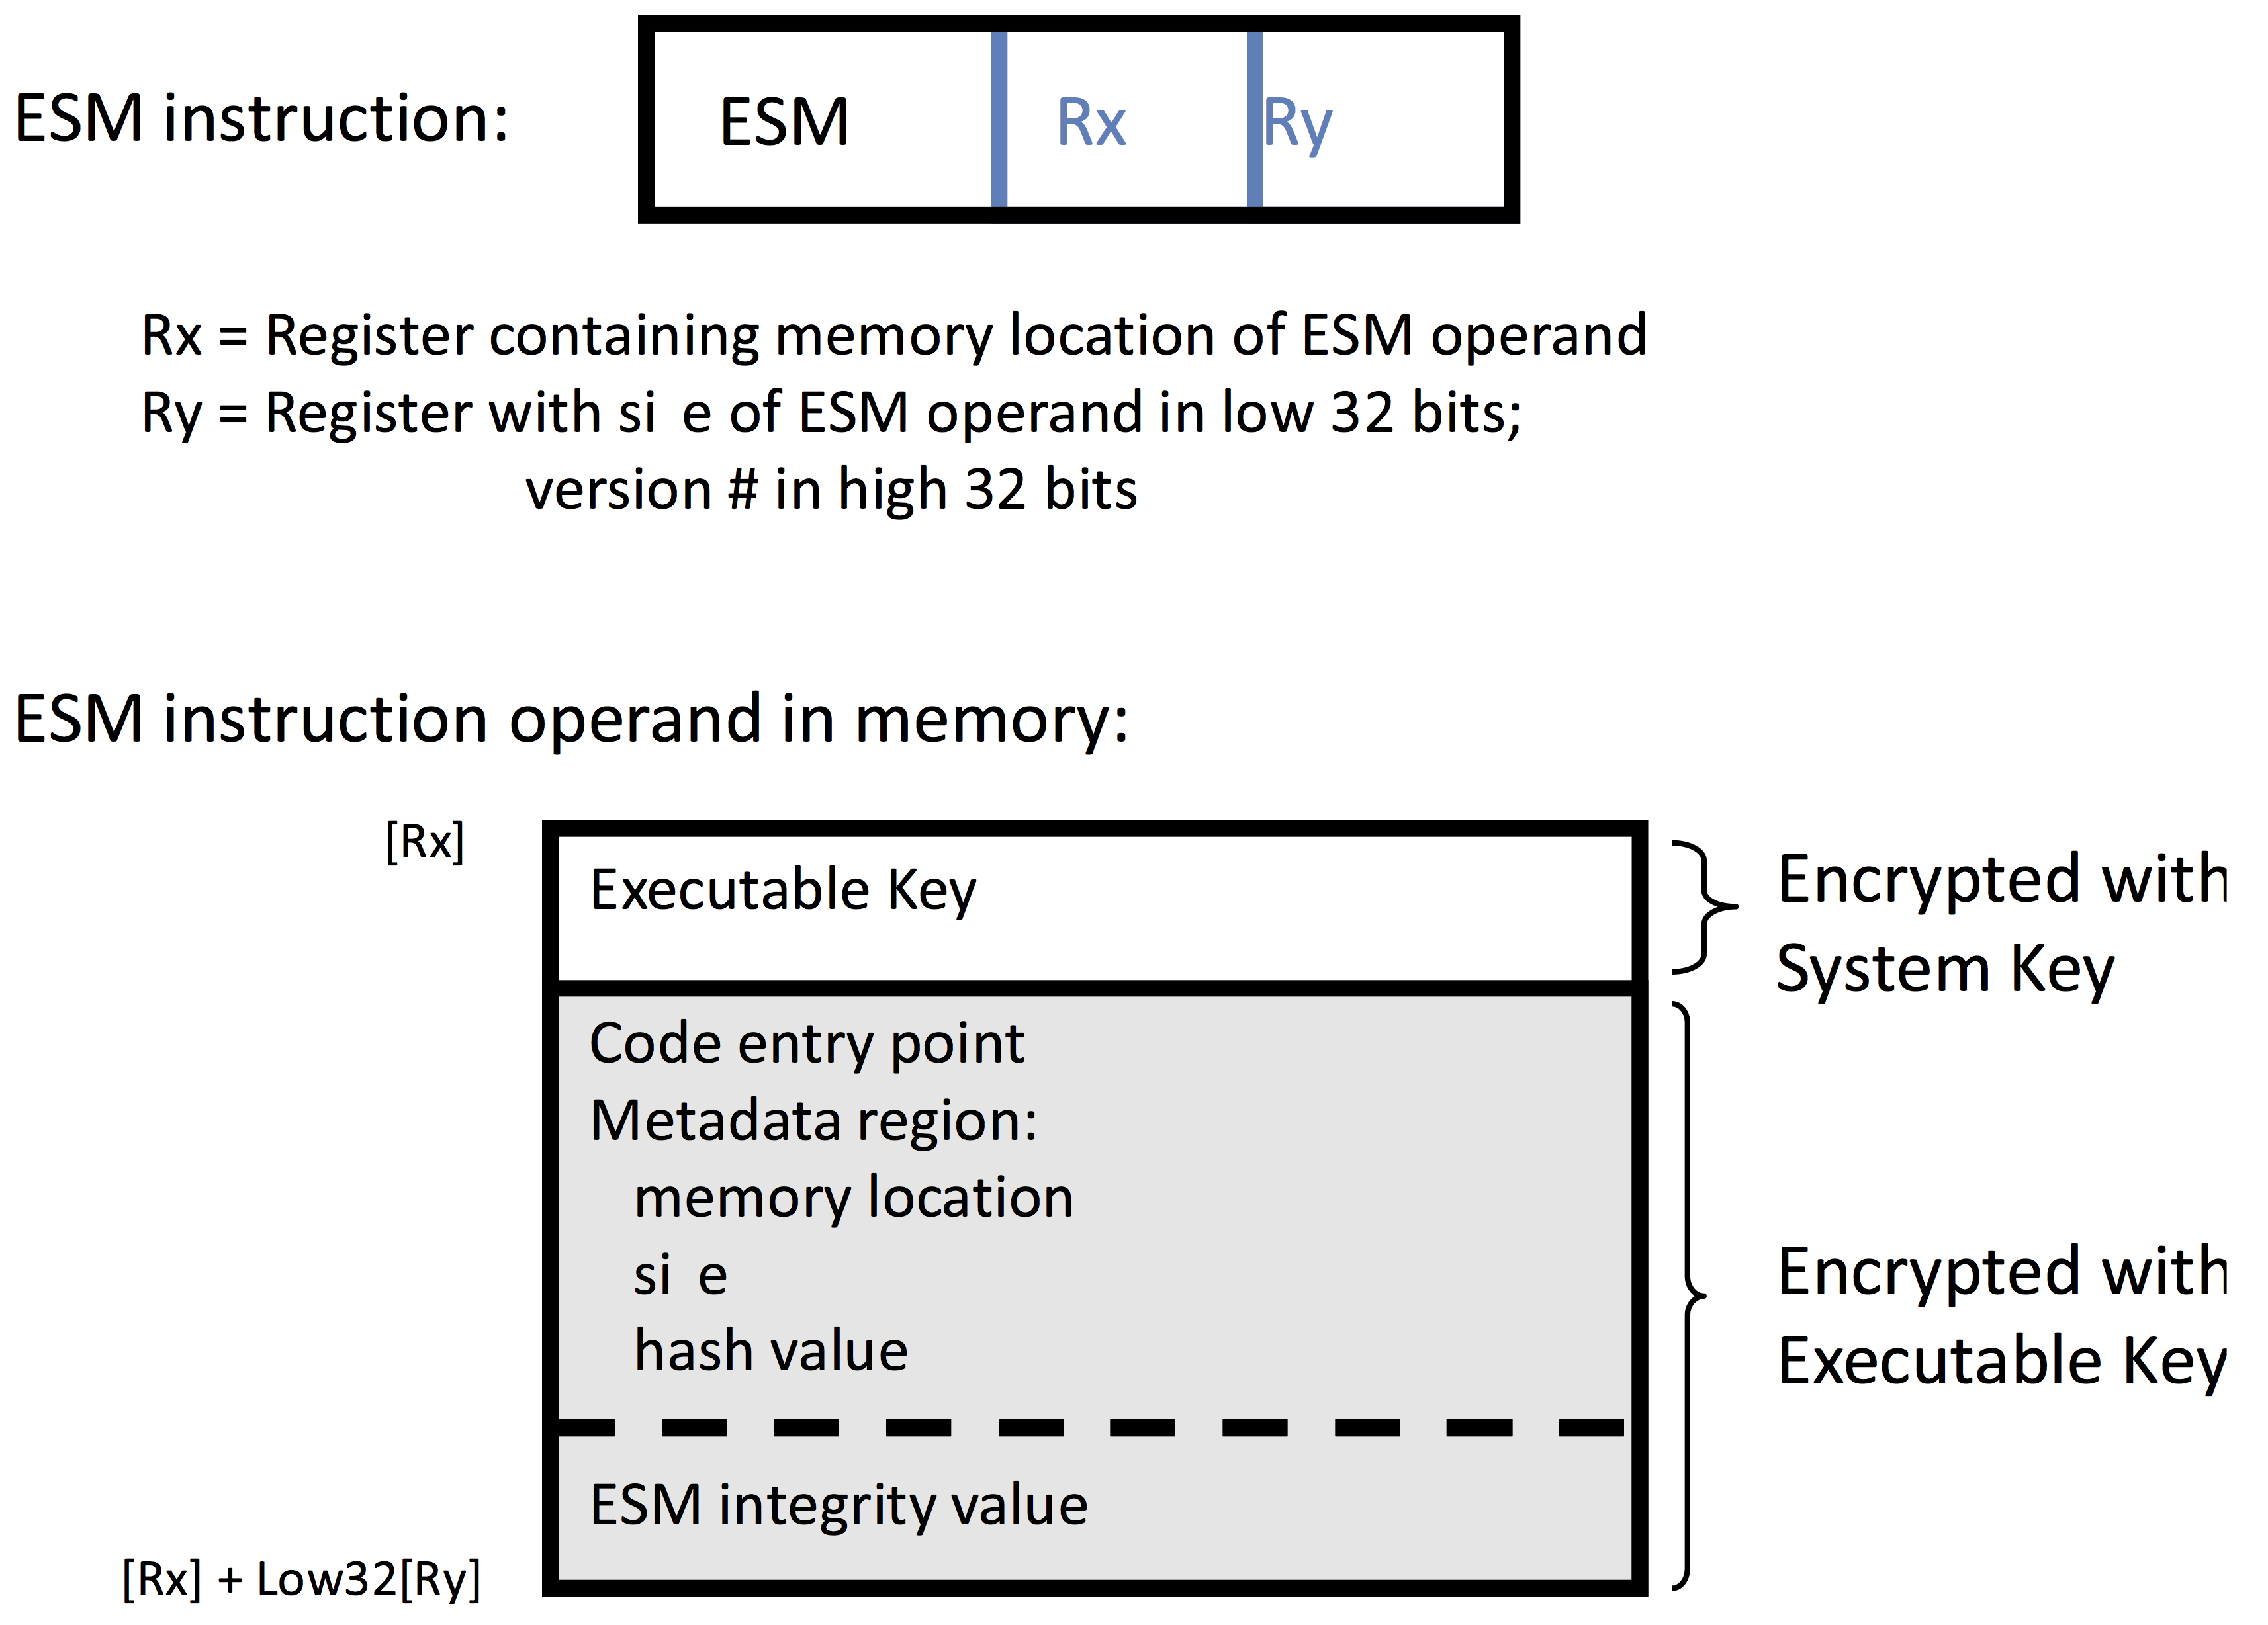
\includegraphics[width=\columnwidth]{esm2}
		\caption{Aufbau der \texttt{esm}-Instruktion}
		\label{fig:esm}
	\end{subfigure}
	\caption{Verschlüsselung und \texttt{esm}-Instruktion \cite{boivie2013secureblue++:big}}
\end{figure}
\label{sec:register}
Zur Umsetzung von SecureBlue++ wurden mehrere neue Register eingeführt. Hierbei existieren, wie in \cref{fig:keys} gezeigt, ein ROM\footnote{Wie genau der öffentliche Schlüssel gelesen werden kann, wurde nicht angegeben.} auf der CPU die Private/Public Keys beinhaltet. Der ROM für den Privaten Schlüssel ist nur innerhalb der \texttt{esm}-Instruktion von der CPU lesbar \cite{boivie2013secureblue++:big,secureblue++patent}.

\paragraph{Secure Executable ID Save/Restore (\texttt{SEIDSR)}}
Das \texttt{SEIDSR}-Register kann nur mit privilegiertem Zugriff ausgelesen werden und gibt die aktuelle \emph{SEID} zurück. Der Inhalt des Registers ist nur mit privilegierten Rechten beschreibbar und wird für die neu eingeführten Instruktionen benötigt.

\paragraph{Secure Executable ID (\texttt{SEID)}}
Die CPU benutzt das \texttt{SEID}-Register (früher auch \texttt{EID}-Register genannt \cite{boiviesecureblue++:small,secureblue++patent}) für die interne Speicherung der aktuell ausgeführten durch SecureBlue++ geschützten Anwendung. Es ist nicht möglich den Wert dieses Registers direkt zu manipulieren oder ihn auszulesen.

\subsection{Neue Instruktionen}
\label{sec:instruktionen}
Es wurden vier neue Instruktionen als Interface eingeführt, damit Applikationen und das zugrunde liegende Betriebssystem die SecureBlue++ Erweiterung benutzen können.
\paragraph{Enable Secure Mode (\texttt{esm})}
\label{sec:esm}
Die \texttt{esm}-Instruktion ist in \cref{fig:esm} aufgezeigt und bekommt eine Konfigurationsstruktur übergeben bei dem das Register \texttt{Rx} den Start und \texttt{Ry} die Größe der Struktur angeben. Die Konfiguration besitzt als erstes Attribut den \texttt{Executable Key}, welcher ein eigens für die Applikation erzeugter AES-Schlüssel ist und nur dieser wird, wie in \cref{fig:keys} gezeigt, mit dem öffentlichen Schlüssel der CPU verschlüsselt. Alle weiteren Attribute sind mit dem \texttt{Executable Key} verschlüsselt. Bei dem \texttt{Code entry point} handelt es sich um einen Zeiger auf die Startfunktion der jeweiligen Applikation, zum Beispiel die \verb|main| Funktion in einem C-Programm. Die \texttt{Metadata region} wird in \cref{sec:metadata} erläutert. Bei der \texttt{ESM integrity value} handelt es sich um einen Hash-Wert der Konfiguration um Manipulationen zu verhindern. Nachdem die Integrität der Konfiguration sichergestellt wurde, wird eine \emph{SEID} generiert, in das \texttt{SEID}- und \texttt{SEIDSR}-Register geschrieben, die Eintragungen in den Verwaltungstabellen erzeugt und das Programm über den \texttt{Code entry point} gestartet.

\paragraph{\texttt{restorecontext}}
Das Betriebssystem muss beim Kontextwechsel zuerst die \emph{SEID} aus dem \texttt{SEIDSR}-Register auslesen und sich diese zusätzlich in der Thread-Verwaltung speichern. Wenn das Betriebssystem eine mit SecureBlue++ geschützte Anwendung wieder aufnehmen, so muss das \texttt{SEIDSR}-Register mit entsprechenden und validen \emph{SEID} belegt und die \texttt{restorecontext}-Instruktion aufgerufen werden. Im Anschluss werden automatisch durch die Hardware die Register und der Status aus der \emph{TRL} wiederhergestellt und die Applikation nimmt ihre Arbeit wieder auf.

\paragraph{\texttt{deletecontext}}
Durch die \texttt{deletecontext}-Instruktion werden alle Ressourcen der durch das \texttt{SEIDSR}-Register bestimmten Anwendung, wie Metadaten, Register und Cache Lines sowie alle Eintragungen in den \emph{Secure Executable Table} und \emph{Protected Memory Table} gelöscht und können nicht mehr mit der \texttt{restorecontext}-Instruktion wiederhergestellt werden. Somit sollte diese Instruktion immer zum Beenden der jeweiligen Anwendung genutzt werden. Es entstehen keine Sicherheitslücken, wenn diese Instruktion durch Angreifer benutzt wird. 

\paragraph{Secure Executable System Call (\texttt{sesc})}
Diese Instruktion wird zwingend für die Umsetzung von System Calls benötigt, weil im Secure-Modus das Verhalten der eigentlichen \texttt{sc}-Instruktion, wie in \cref{fig:sesc} dargestellt, verändert wurde. Weitere Informationen zur Funktionsweise der \texttt{sesc}-Instruktion folgt in \cref{sec:sesc}.

\subsection{System Calls}
\begin{figure}
	\centering
	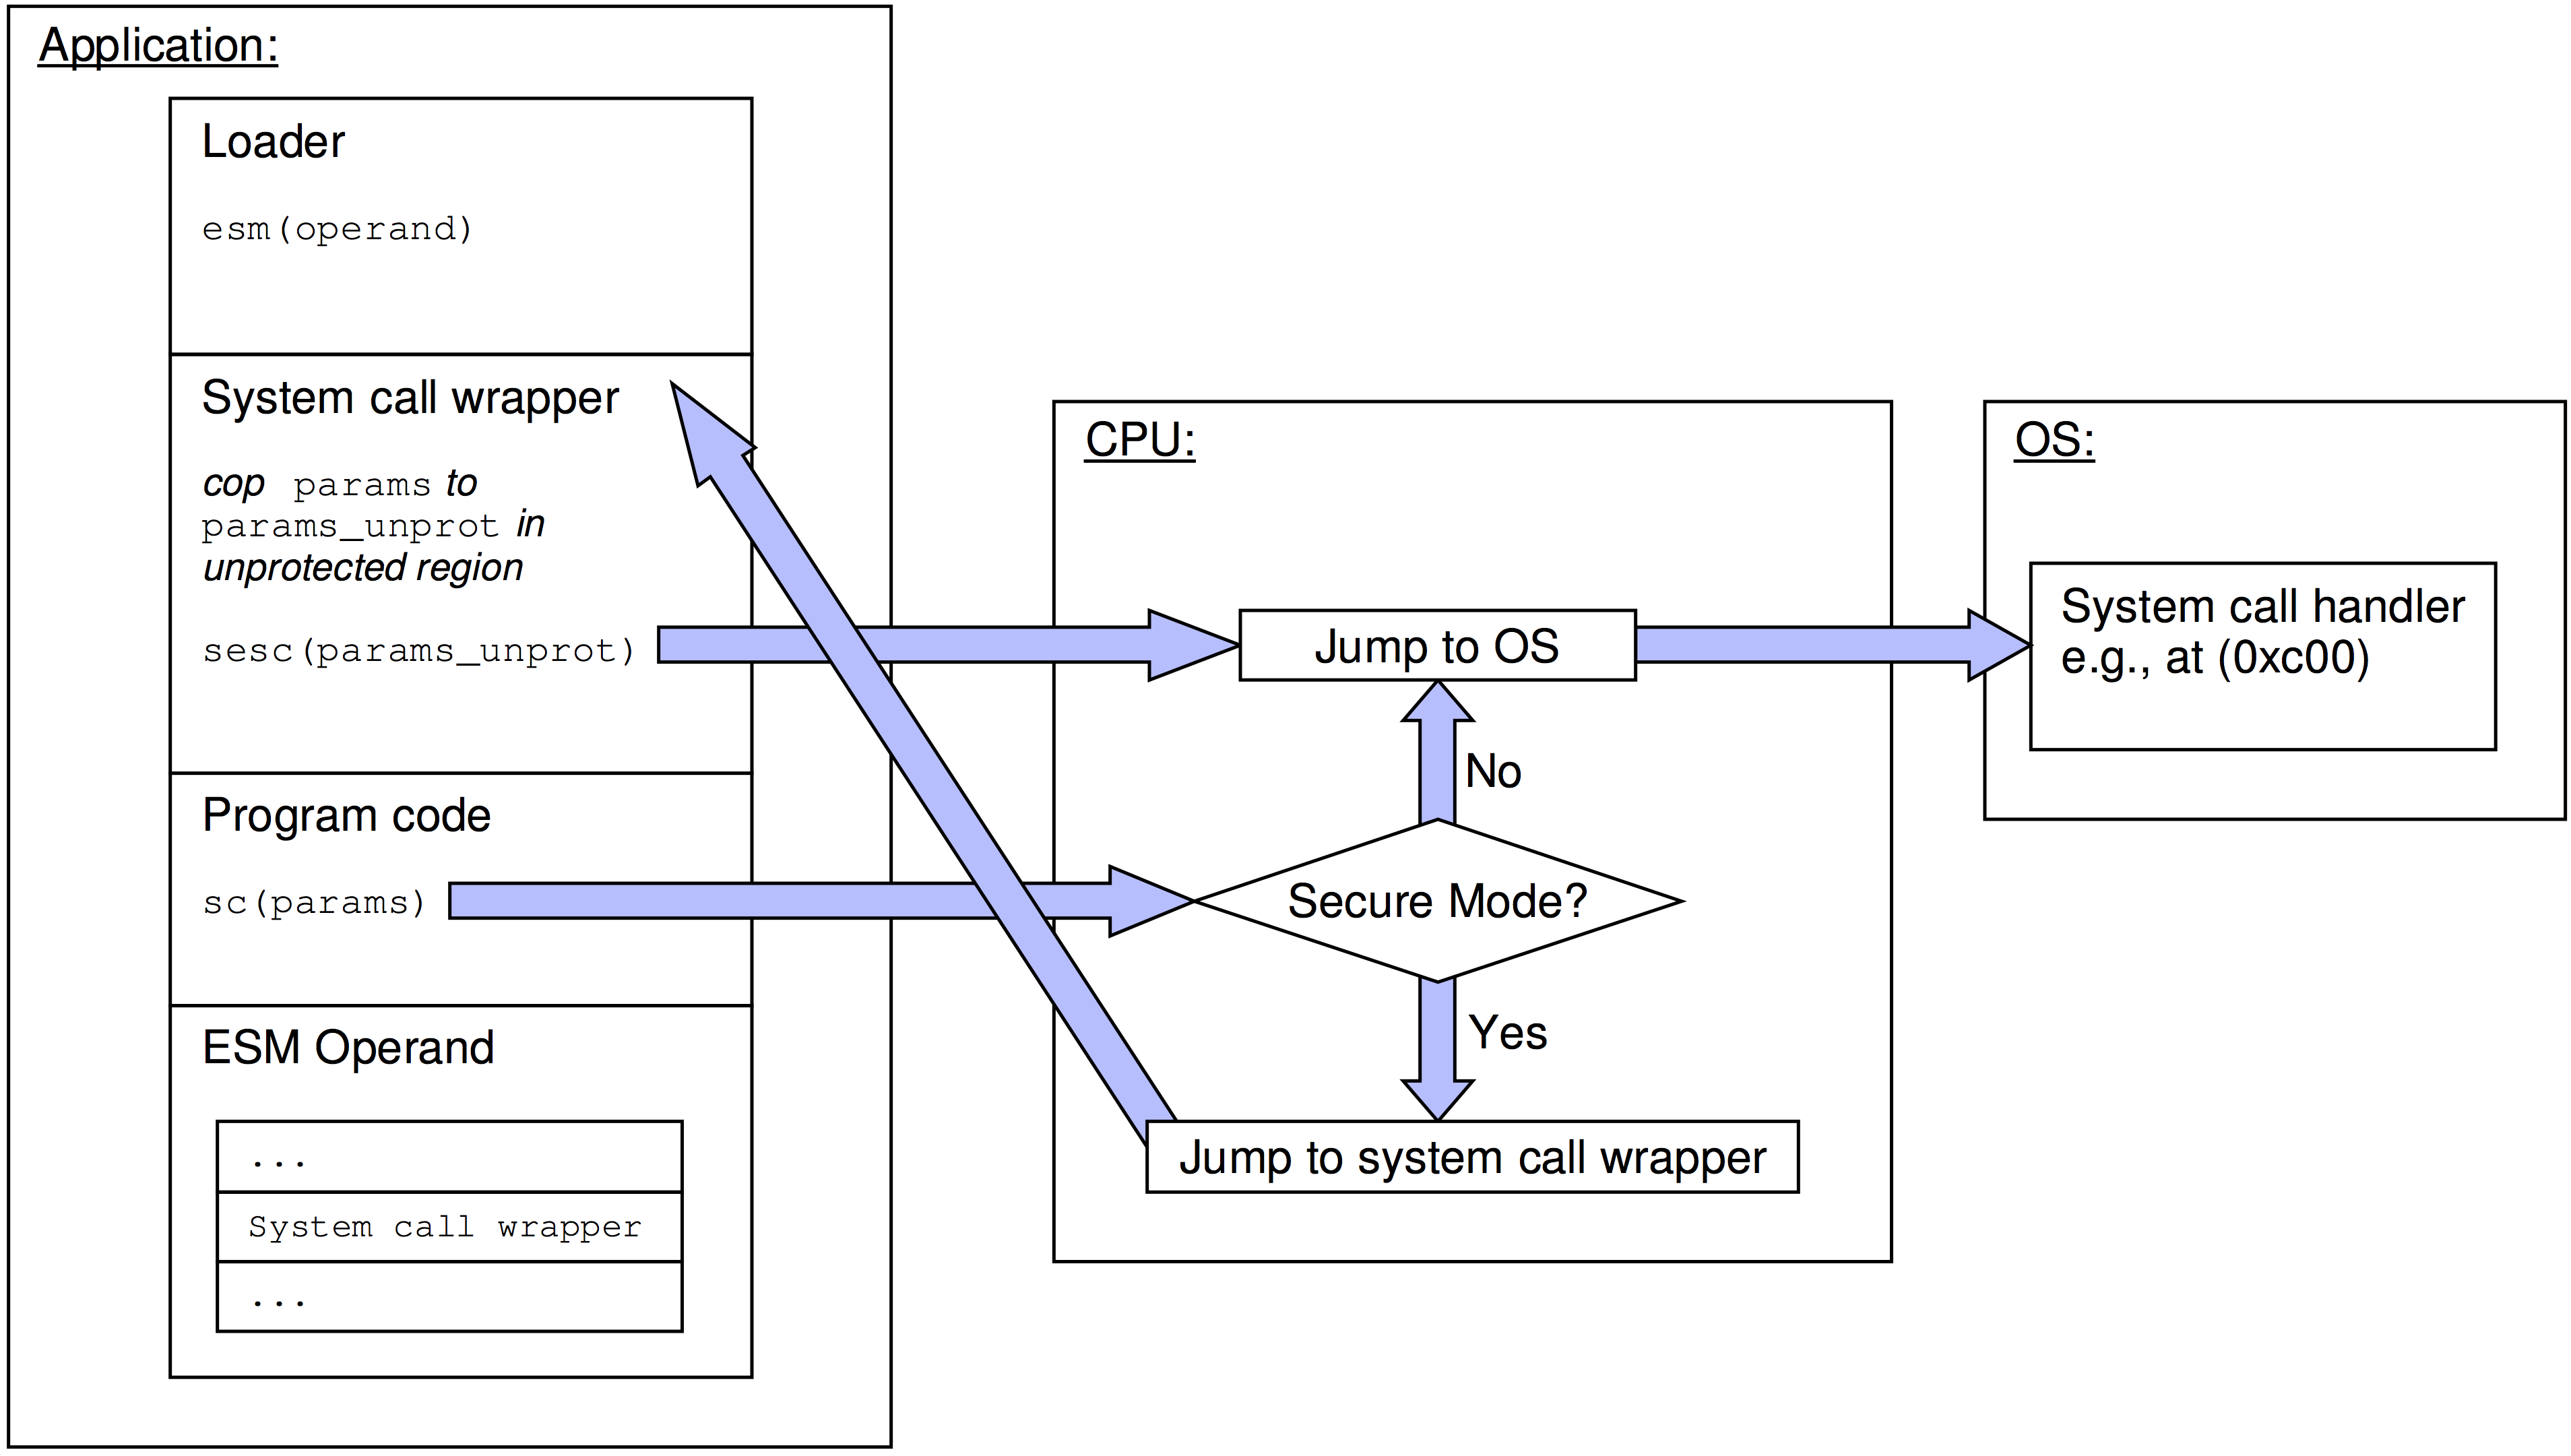
\includegraphics[width=\columnwidth]{sesc2}
	\caption{Grundidee: Die \texttt{sc}-Instruktion wird im Secure-Modus von einem eigenen Handler abgefangen und verarbeitet. \cite{boivie2013secureblue++:big}}
	\label{fig:sesc}
\end{figure}
\label{sec:sesc}
System Calls dienen als Interface für Anwendung mit dem jeweiligen Betriebssystem. Jedoch ist nach dem Bedrohungsszenario aus \cref{sec:bedrohungsszenario} das Betriebssystem mit den dazugehörigen Interrupt Handlern als nicht vertrauenswürdig zu erachten und muss aus diesem Grund aus der \emph{trusted computin base} \emph{TCB} ausgeschlossen werden. Des weiteren müssen die Rückgabewerte von System Calls auf ihre Sinnhaftigkeit überprüft werden, um gegen Iago Attacken abgesichert zu sein \cite{checkoway2013iago}.

Bei jedem Aufruf der \texttt{sc}-Instruktion wird von der CPU überprüft, ob sich die Applikation im Secure-Modus befindet oder nicht. Ist der Secure-Modus nicht aktiviert wird der System Call Handler des Betriebssystems aufgerufen und die Abarbeitung des System Calls erfolgt wie gewohnt durch einen System Call Interrupt. Ist die Anwendung jedoch im Secure-Modus wird ein eigener in der Applikation vorhandener System Call Handler aufgerufen. Dieser kopiert die Daten aus der dem geschützten Arbeitsspeicher in ungeschützte Regionen und führt im Anschluss mit dem \texttt{sesc}-Interrupt den System Call aus. Nach der Beendigung des System Calls werden die Ergebnisse auf Sinnhaftigkeit überprüft und in den gesicherten Arbeitsspeicher überführt. 

Aus Performance-Gründen wird beim \texttt{sesc}-Interrupt der Register-Schutz ausgeschaltet, weswegen der System Call Wrapper die Register für die Übergabe von Werten verwenden kann aber sich selbst für die Sicherheit der Daten kümmern muss, um nicht versehentlich Geheimnisse zu verraten \cite{boivie2013secureblue++:big}. Durch diese Umsetzung von System Calls müssen keine Änderungen am Quellcode der Anwendung oder der zugrunde liegenden Bibliotheken, wie der libc, vorgenommen werden. Jedoch können nicht alle System Calls mit dieser Art Wrapper durch geführt werden, da manche entweder den geschützten Speicher der Anwendung manipulieren oder den Status der Register verändern.

\paragraph{\texttt{signal}}
Das Betriebssystem hat bei durch SecureBlue++ geschützten Applikationen keine Möglichkeiten das \texttt{Program Counter}-Register zu verändern. Somit ist es nicht mehr Möglich, dass das Betriebssystem wie üblich den \texttt{PC} auf den gewünschten Signal Handler zu verschiebt. Um den \texttt{signal} System Call trotzdem zu unterstützen, wird beim Aufruf der \texttt{esm}-Instruktion ein übergeordneter Handler registriert, der auf Anwendungsebene die jeweils gewünscht Aktion ausführt \cite{boivie2013secureblue++:big}. Damit kann das Betriebssystem höchstens eines der angebotenen Aktionen von der Anwendung ausführen lassen und keine anderen für das Programm möglicherweise gefährlichen Aktionen. Die Umsetzung des Signal Handlers ist für das Betriebssystem völlig transparent.

\paragraph{\texttt{fork}}
Der \texttt{fork} System Call kann nicht über das Betriebssystem ausgeführt werden, da das Betriebssystem keinen lesenden Zugriff auf die jeweiligen Speicherbereiche besitzt. Deswegen wird durch den Wrapper einen Signal an die Applikation gesendet, welches die Anwendung veranlasst seinen benutzen Speicher selbst zu duplizieren und diesem im Anschluss einem neuen mit SecureBlue++ gesichertem Prozess zu zuweisen.

\paragraph{\texttt{clone}}
Um Multi-threading zu ermöglichen ist eine Unterstützung des \texttt{clone} System Calls zwingend erforderlich. Wie auch \texttt{fork} benötigt \texttt{clone} eine Unterstützung durch die gesicherte Anwendung. Weitere Informationen hierzu folgen in \cref{sec:multithreading}.

\paragraph{\texttt{exit}}
Damit keine Geheimnisse aus einer beendeten Anwendung entweichen können, wird das Programm nach dem Aufruf von \texttt{exit} in eine Endlosschleife aus \texttt{nop}-Instruktionen versetzt. Hierdurch wird verhindert das nach der Beendigung der Anwendung irgendwelche potenziell gefährlichen Aktionen ausgeführt werden. 

\subsection{Umsetzung über Software}
Neben dem System Call Wrapper gibt es weitere durch Software umgesetzte Funktionalitäten mit deren Hilfe SecureBlue++ eine gesicherte Ausführung von Anwendungen ermöglicht. Diese Bestandteile werden in die zu sichernde Anwendung statisch hinein kompiliert. 

\paragraph{Integrity Tree}
\label{sec:Integritätsbaum}
Der Integrity Tree dienst neben der Verschlüsselung zum Schutz des Arbeitsspeichers vor Manipulationen. Der Baum ist nach dem Key/Value-Prinzip aufgebaut, bei dem jede zu schützende Cache Line auf einen Hashwert in den Blättern abgebildet wird. Die Knoten des Baumes schützen immer ihre Kindknoten vor Manipulationen durch das Abbilden von Kindknoten auf Hash-Werte. Um den Baum möglich flach zu halten, kann jeder Knoten acht Kindknoten beherbergen und schützen. Cache Lines, die im Cache verändert wurden, werden Markiert und erst wenn diese aus dem Cache entfernt werden sollen in den Baum zurück geschrieben. Hierbei muss jedoch vom Blatt an alle Elternknoten ebenfalls mit aktualisiert werden, da die Elternknoten die Hash-Werte der Kindknoten mit überwachen.

\paragraph{Metadata}
\label{sec:metadata}
Die Metadaten einer gesicherten Anwendung werden durch den Integrity Tree geschützt, bei jedem wieder Aufruf der Anwendung neu in den Cache geladen sowie validiert und werden in der so genannten \emph{Metadaten Region} gespeichert. Der Zustand wird, wie in \cref{fig:esm} aufgezeigt, beim Aufruf der \texttt{esm}-Instruktion übergeben. Die Metadaten bestehen unter anderem aus den Signal Handlern, die bei der \texttt{singal}-Instruktion aufgerufen werden, die hinein kompilierten System Call Wrapper und der \emph{die Memory Region Mapping Table} (\emph{MRMT}). Des weiteren beinhalten die Metadaten die Adresse der \emph{TRL}.

\paragraph{Secure Executable Table}
Bei der \emph{Secure Executable Table} (\emph{SET}) handelt es sich um eine nur in der CPU\footnote{\label{foot:ungenau}Die genaue Position wurde bisher nicht genau bekannt gegeben.} befindliche Datenstruktur, welche alle aktiven gesicherten Anwendungen beinhaltet und nur durch die CPU mit den neu eingeführten Instruktionen geändert werden kann. Die Größe der \emph{SET} ist hardwareseitig limitiert\footnote{Die genaue Größe wurde bisher nicht spezifiziert.} und hierdurch ist ebenfalls die maximale Anzahl von gleichzeitig zu benutzenden durch SecureBlue++ gesicherten Anwendungen limitiert. Jeder Eintrag besteht aus den diesen Eigenschaften:
\begin{itemize}
	\item Secure Executable ID (\emph{SEID})
	\item Hash-Wert der Metadaten zur Validierung
	\item Zeiger auf Metadaten Region im Speicher
\end{itemize}

\paragraph{Memory Region Mapping Table}
Die \emph{MRMT} ermöglicht die gesicherte Anwendung eine bei Cache Misses für  schnelle Zuordnung von \emph{MRID}s auf die jeweiligen Speicherbereiche mit dem dazugehörigem AES-Schlüssel. Alle Informationen dieser Tabelle können ebenfalls aus der \emph{Protected Memory Table} (\emph{PMT}) ausgelesen werden, ermöglicht die \emph{MRMT} das Teilen von Speicherbereichen für das Multi-threading. Die Tabelle ist eine \enquote{read-only} Datenstruktur und jeder Eintrag besitzt die folgenden Attribute:
\begin{itemize}
	\item Angaben zum Start und Größe der Region im Speicher.
	\item Der jeweilige AES-Schlüssel für die Region, da jede Region bei geteiltem Speicher von mehreren Anwendungen benutzt werden könnte.
	\item Die Memory Region ID (\emph{MRID}) zur Bestimmung der jeweiligen Region in der \emph{PMT}.
\end{itemize}

\paragraph{Protected Memory Table}
Diese Tabelle ist nur indirekt über die neuen Instruktionen manipulierbar und hält alle Verwaltungsinformationen zu den einzelnen gesicherten Speicherbereichen aller gesicherten Anwendungen in der CPU\cref{foot:ungenau} vor. Grundsätzlich hat jede Anwendung Zugriff auf die verschlüsselten Speicherbereiche, so lange der jeweilige AES-Schlüssel bekannt ist. Anwendungen mit einer passenden \emph{SEID} in \emph{SEID1} oder \emph{SEID2} haben lesenden Zugriff auf die jeweilige Zeile und können somit den AES-Schlüssel abfragen. Jeder dieser Zeilen besteht unter anderem aus den folgenden Daten:
\begin{itemize}
	\item Memory Region ID (\emph{MRID})
	\item \emph{SEID} des Erstellers als \emph{SEID1}
	\item Eine weitere \emph{SEID} als \emph{SEID2}
	\item Statuswert um die Region auf \enquote{read-only} zu stellen
	\item Größe und Start der Region
	\item AES-Schlüssel zur Region
\end{itemize}

\paragraph{Thread Restore List}
In der \emph{TRL} werden hardwareseitig die Registerzustände im  bei einem Interrupt gespeichert und durch den Aufruf der \texttt{restorecontext}-Instruktion wiederhergestellt. Nach dem Wiederherstellen eines Kontextes wird der Eintrag als benutzt markiert und kann nicht erneut wiederhergestellt werden.

\subsection{Multi-threading}
\label{sec:multithreading}
Multi-threading ist in der heutigen Zeit nicht mehr weg zu denken und muss deshalb für geschützte Anwendungen zur Verfügung stehen. Beim Multi-threading bestehen zwei verschiedene Varianten die jeweils unterschiedliche Vor- und Nachteile besitzen und durch SecureBlue++ anders behandelt werden müssen.

\paragraph{User Threads}
User Level Threads werden auf Benutzerebene implementiert und durch einen eigenen Dispatcher verwaltet und ausgeführt. Aus diesem Grund kann der Kenerl Scheduler nicht die einzelnen User Level Threads verwalten, weswegen keine echte Nebenläufigkeit unterstützt wird. Da der Dispatcher selbst von der Anwendung stammt, kann ein angepasster Scheduler mit in die Anwendung kompiliert werden. Hier durch müssen keine weiteren Änderungen am Programm, für die Unterstützung von Multi-threading, vorgenommen werden. 

\paragraph{Kernel Threads}
Diese Art von Threads werden durch den Kernel verwaltet und ausgeführt. Hierfür wird eine Unterstützung durch die CPU benötigt, da für eine gesicherte Anwendung mehrere Kontexte durch die unterschiedlichen Threads verwaltet werden müssen. Normalerweise werden Threads mit dem \texttt{clone} System Call erstellt. Hierfür stellt SecureBlue++ einen POSIX kompatiblen Wrapper zur Verfügung, weil die Betriebssystem eigene Implementierung keinen Zugriff die \emph{TRL} besitzt. Beim Aufruf von \texttt{clone} wird ein neuer Eintrag in der \emph{TRL} mit den entsprechenden Statuswerten angelegt. Des weiteren ist es dem Kernel Scheduler möglich zwischen den verschiedenen noch nicht gestarteten in der \emph{TRL} gespeicherten Kontexten auszuwählen.

\subsection{Virtuelle Maschinen}
\label{sec:vms}
\begin{figure}
	\centering
	\begin{subfigure}[b]{0.48\columnwidth}
		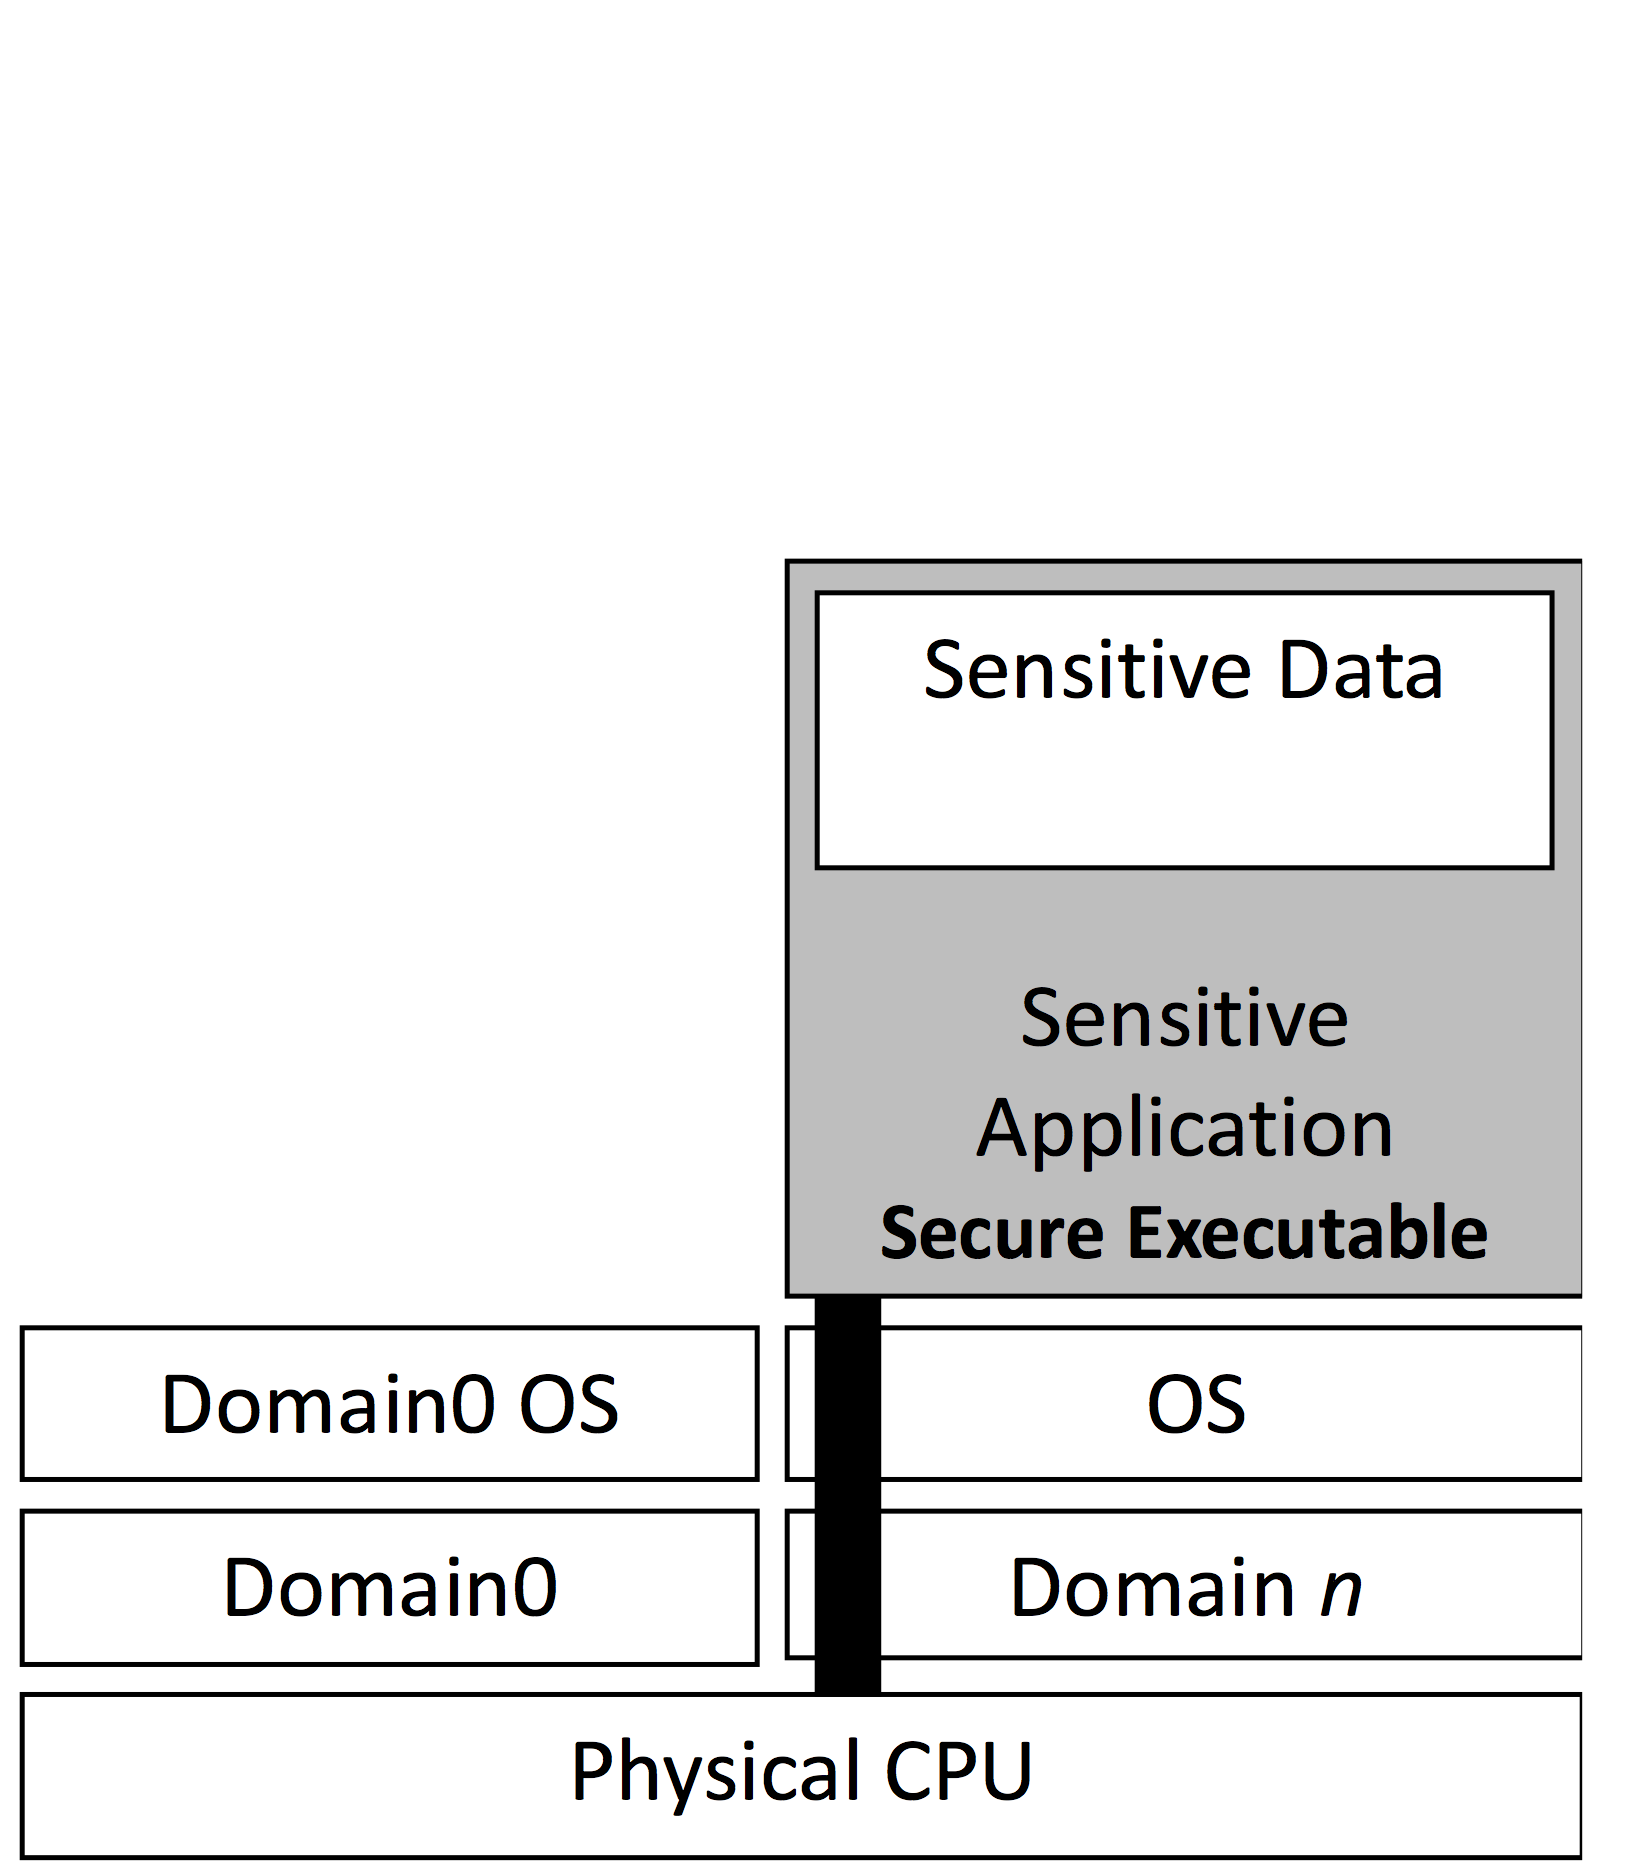
\includegraphics[width=\columnwidth]{hvm2}
		\caption{Hardware VM}
		\label{fig:hvm}
	\end{subfigure}
	\hfill
	\begin{subfigure}[b]{0.48\columnwidth}
		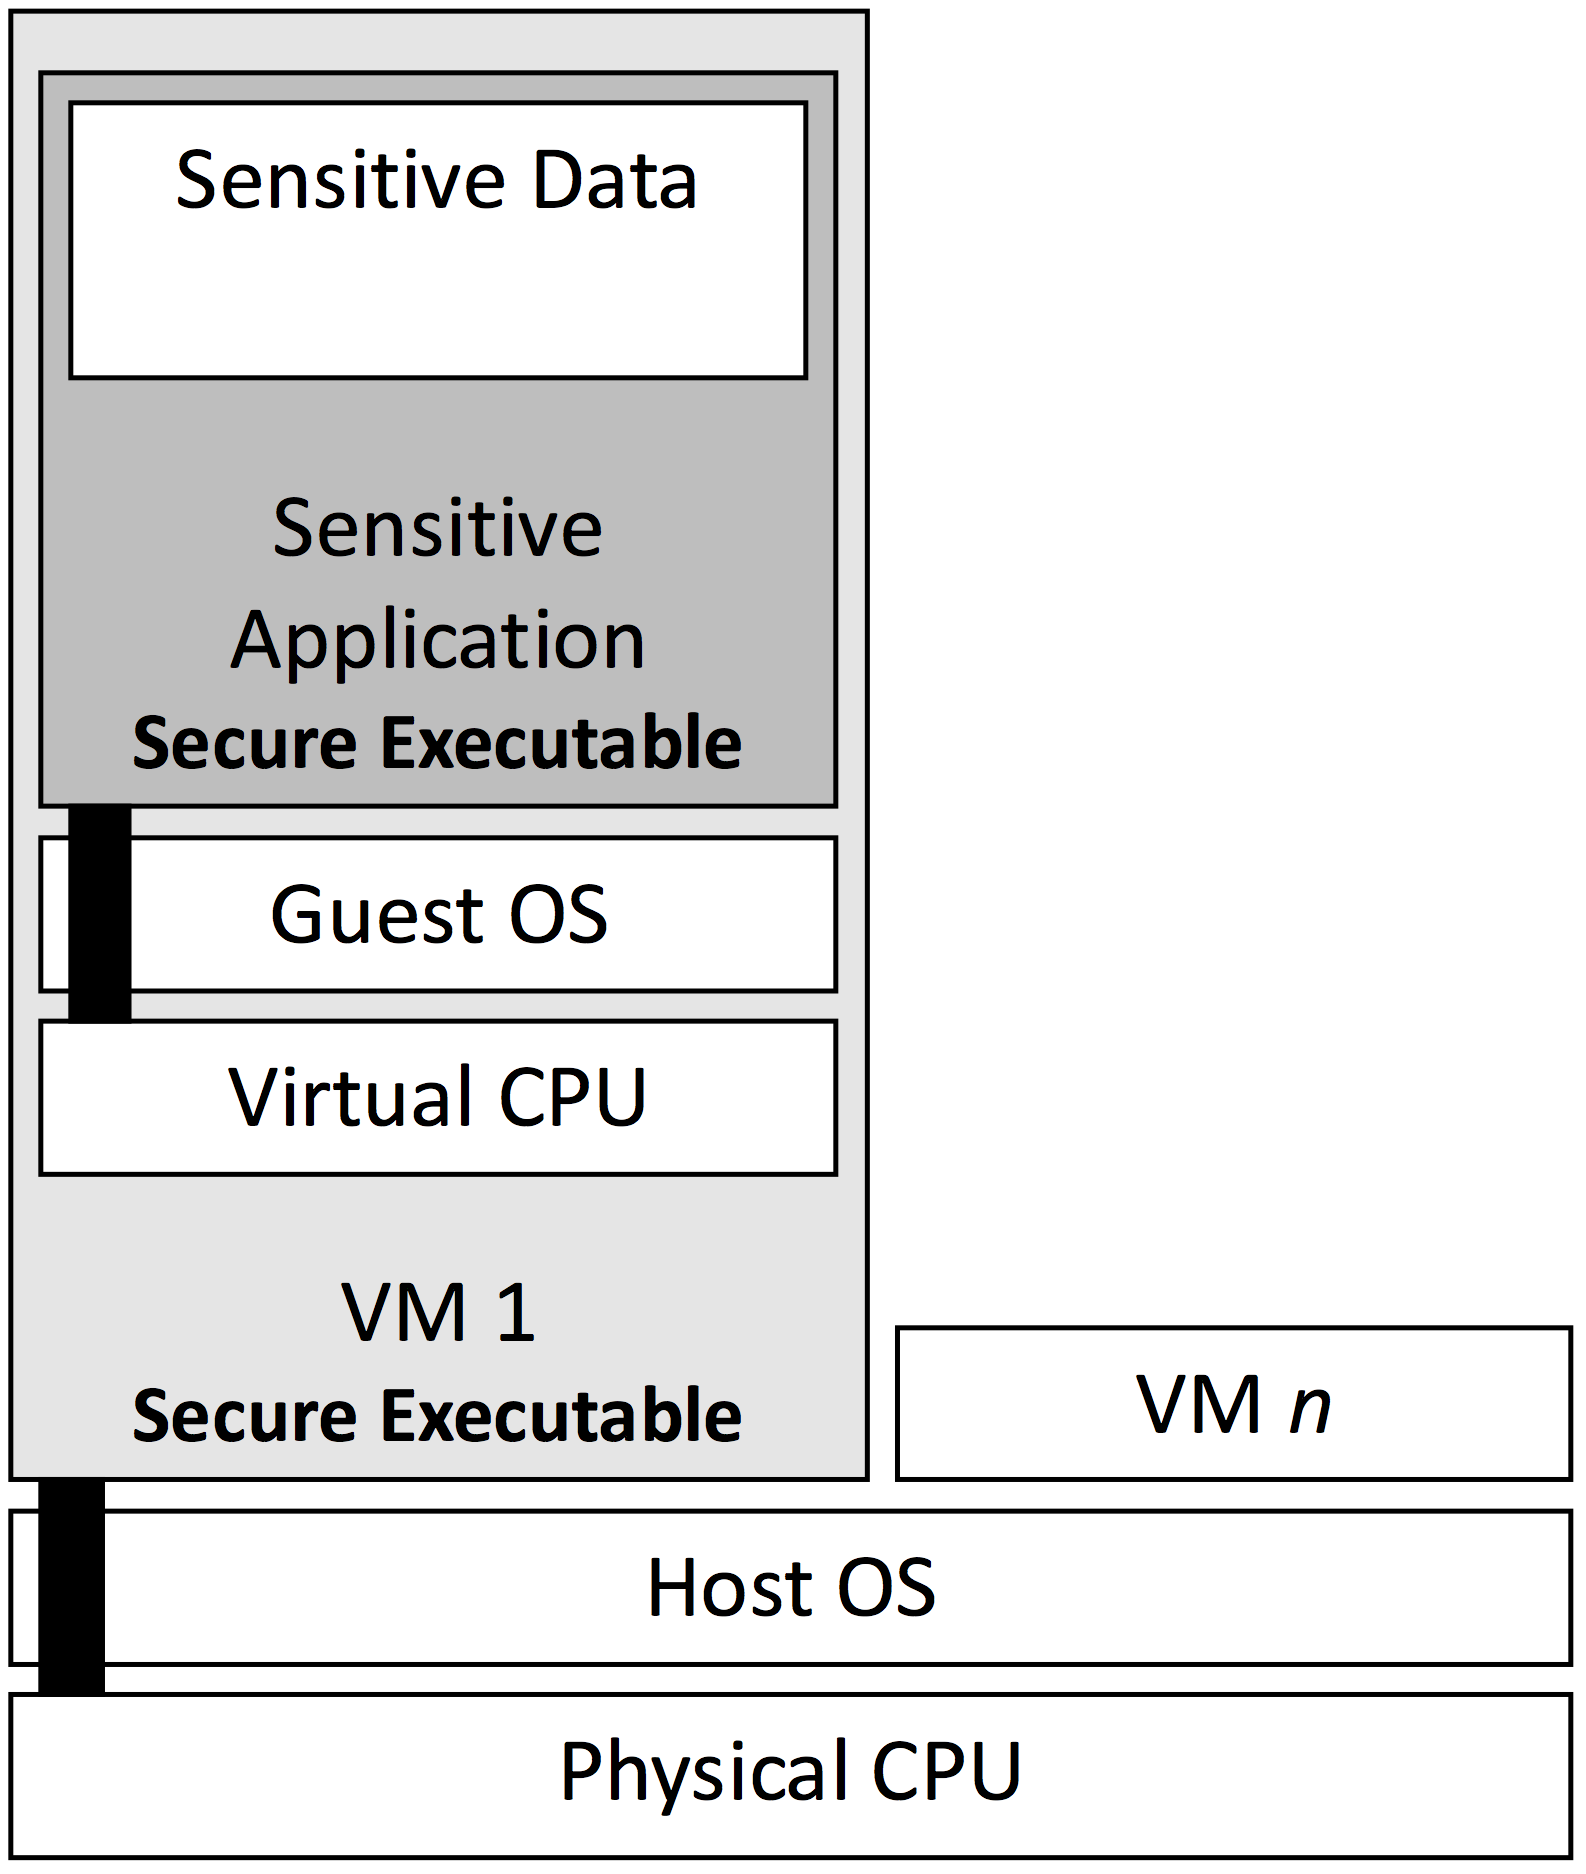
\includegraphics[width=\columnwidth]{svm2}
		\caption{Software VM}
		\label{fig:svm}
	\end{subfigure}
	\caption{Arten von VMs \cite{boivie2013secureblue++:big}}
	\label{fig:vms}
\end{figure}
SecureBlue++ wurde designt um mit Soft- und Hardware basierten virtuellen Maschinen, die in \cref{fig:vms} aufgezeigt sind, zusammenzuarbeiten. 

\paragraph{Hardware VMs}
bei Hardware VMs oder auch \enquote{bare-metal VMs} genannt, handelt es sich um VMs ohne einen Softwarehypervisor, welcher die privilegierten Instruktionen des Gastsystems (in \cref{fig:hvm} Domain $n$) abfängt. Somit verhält sich eine Hardware VM wie ein normales System und kann genauso Applikationen die mit SecureBlue++ gesichert sind ausführen. Für IBM ist diese Art der VM die eigentliche Zielgruppe, da diese am weit verbreiteten im high-performance Sektor sind. Wie bei normalen System muss nur die jeweilige Applikation innerhalb der \emph{TCB} liegen und das Betriebssystem der VM muss nicht vertraut werden. Das Domain $0$ System startet bzw. stellt die gesicherte Anwendung wieder her indem es die \texttt{restorecontext}-Instruktion mit der jeweiligen \emph{SEID} aufruft. Um an die \emph{SEID} zu kommen, muss das Domain $0$ System bei einem Hypervisorinterrupt das \texttt{SEID}-Register auslesen.

\paragraph{Software VMs}
Im Gegensatz zu Hardware VMs besitzen Software VMs einen Softwarehypervisor, der die privilegierten Instruktionen des Gastsystems abfängt und an das gastgebende System weiterleitet und ausführen lässt. Dieser Umstand zwingt einen anderen Ansatz als bei Hardware VMs, da fast alle neuen Instruktionen aus \cref{sec:instruktionen} privilegiert sind und deswegen der Softwarehypervisor Zugriff auf die geschützte Anwendung benötigt. Aus diesem Grund muss das Gastsystem, wie in \cref{fig:svm} gezeigt, in eine gesicherte Anwendung überführt werden. Somit muss jedes System das Instruktionen emuliert in die \emph{TCB} mit aufgenommen werden, jedoch muss das gastgebende System nicht in die \emph{TCB} aufgenommen werden. Dennoch kann die Applikation vom Gastsystem geschützt werden, in dem die zu sichernde Anwendung in eine virtuelle Secure Executable  überführt wird. Hier durch wird das Gastsystem vor dem gastgebenden System geschützt sowie die Anwendung vor beiden Systemen. 

\section{Benchmark}
\begin{figure}
	\centering
	\begin{subfigure}[b]{0.48\columnwidth}
		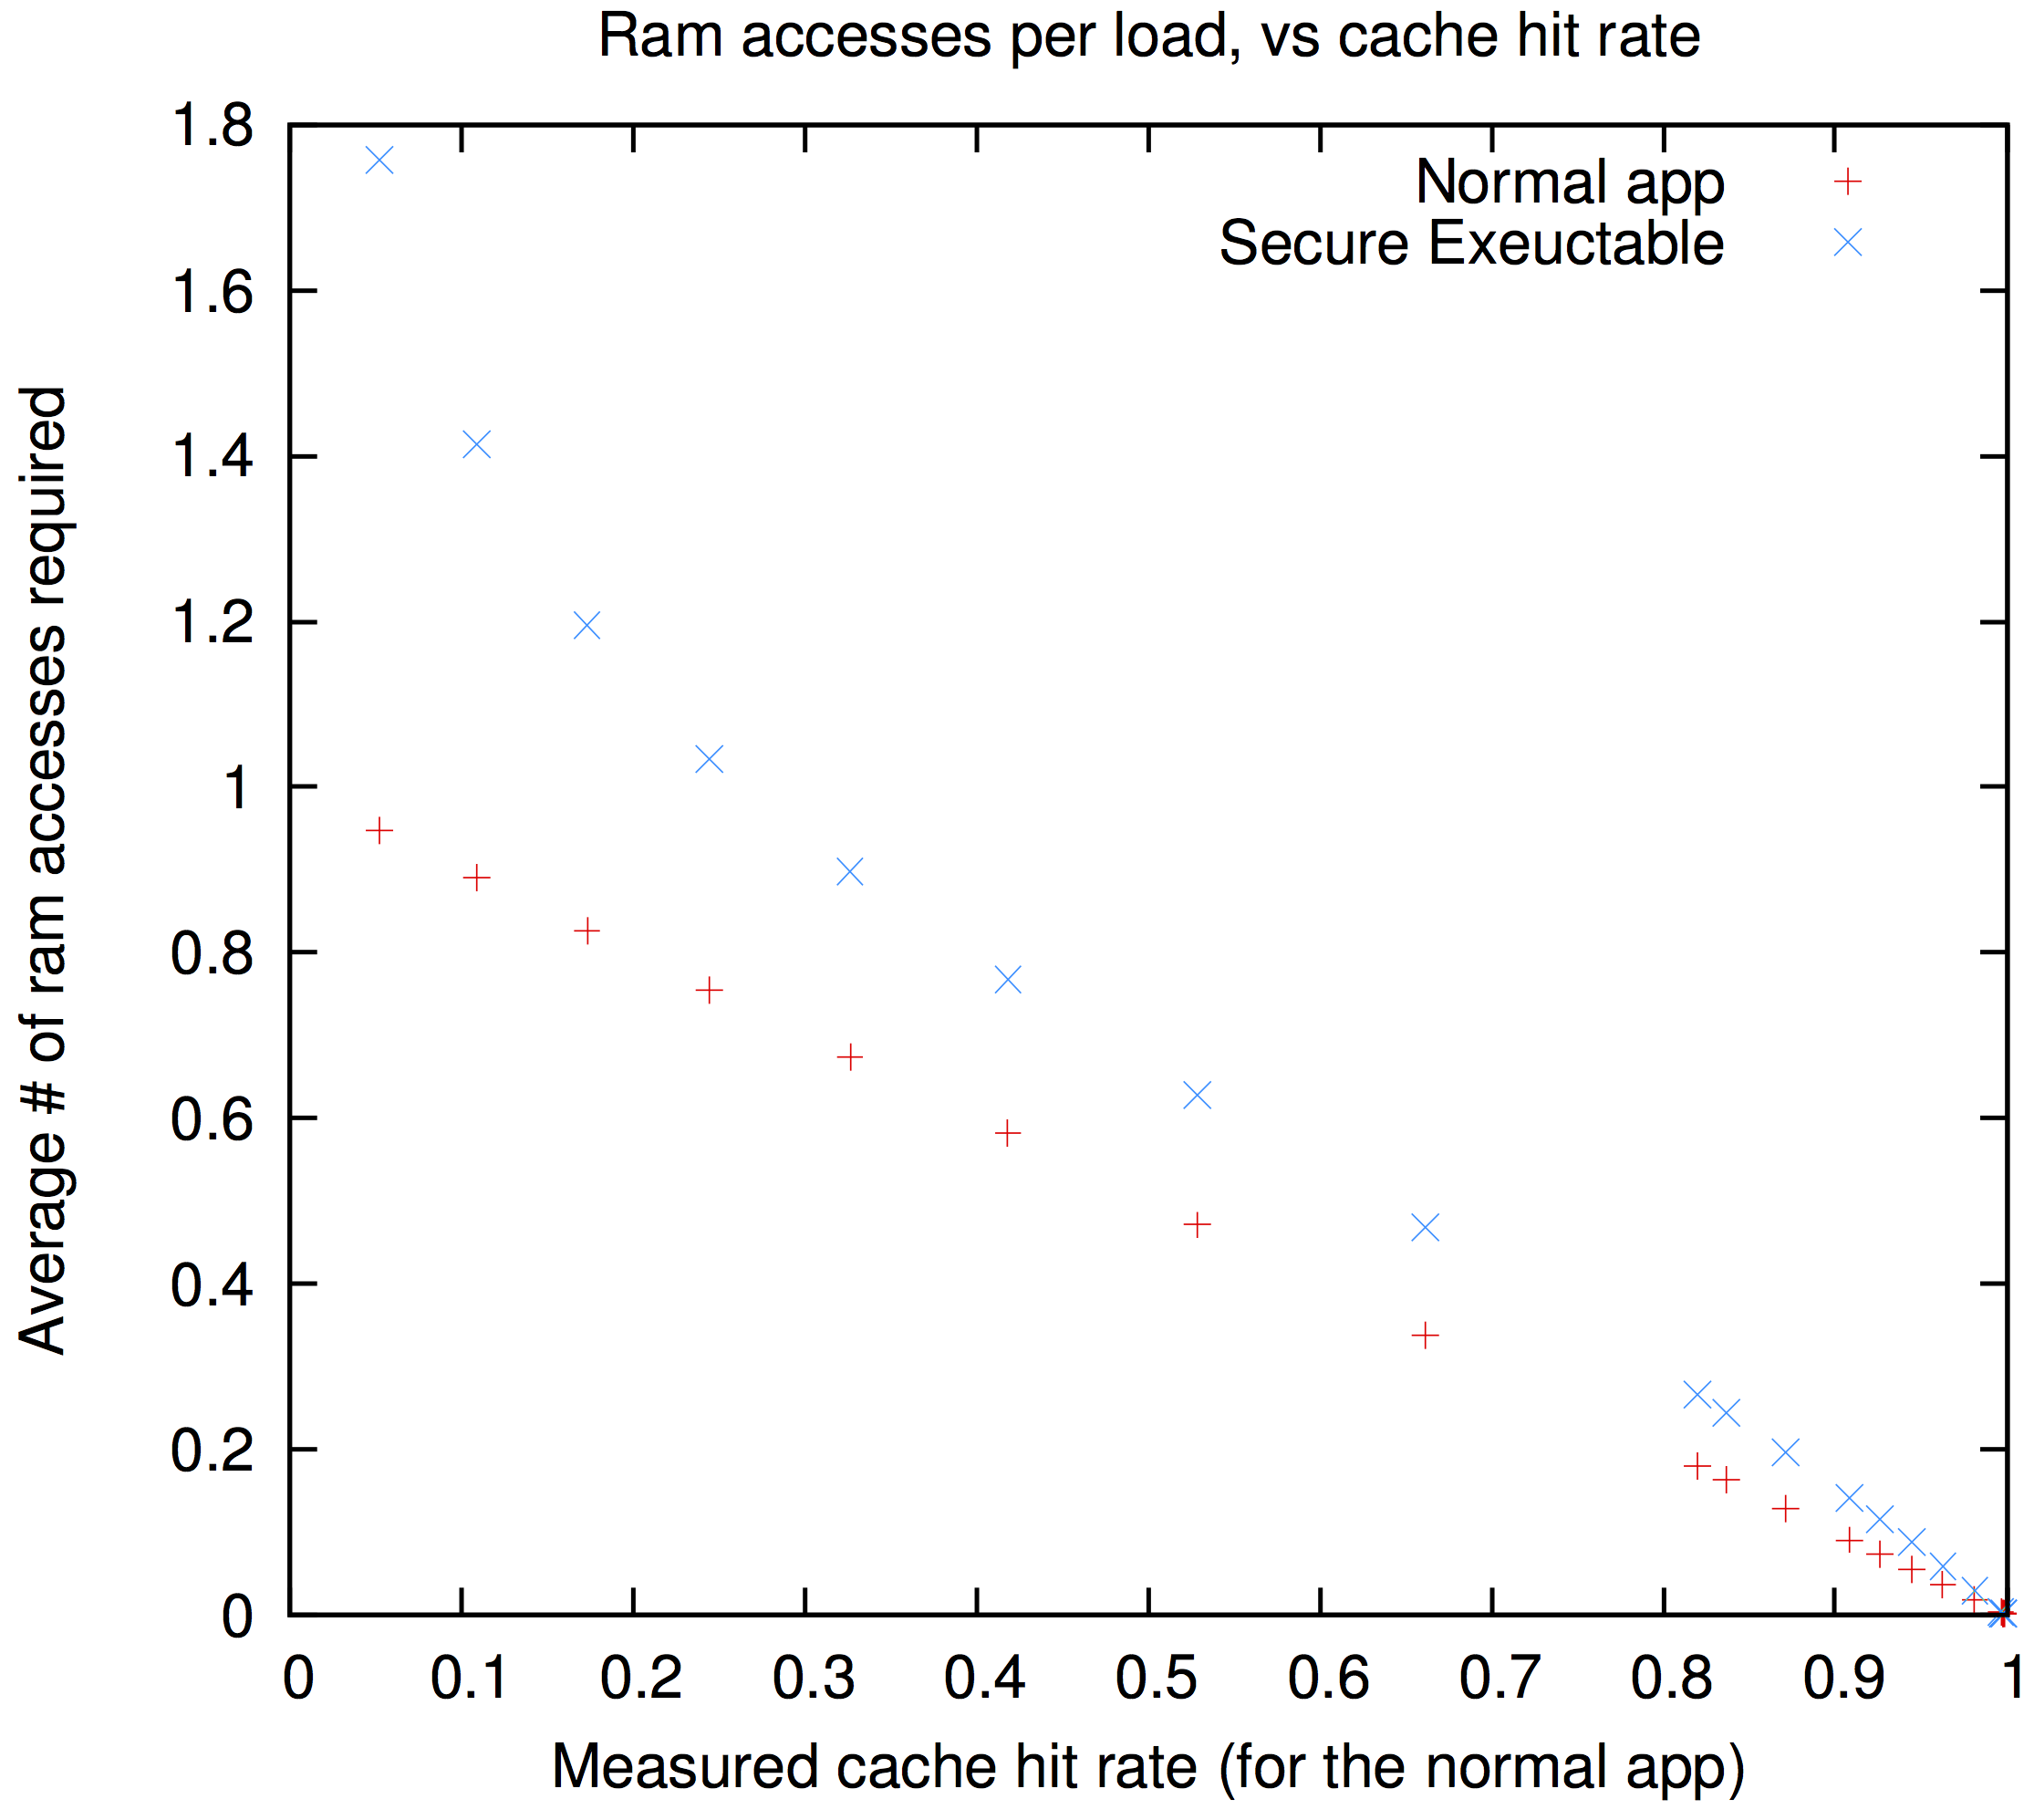
\includegraphics[width=\columnwidth]{bench_per_load2}
		\caption{Lesen}
		\label{fig:bench_load}
	\end{subfigure}
	\hfill
	\begin{subfigure}[b]{0.48\columnwidth}
		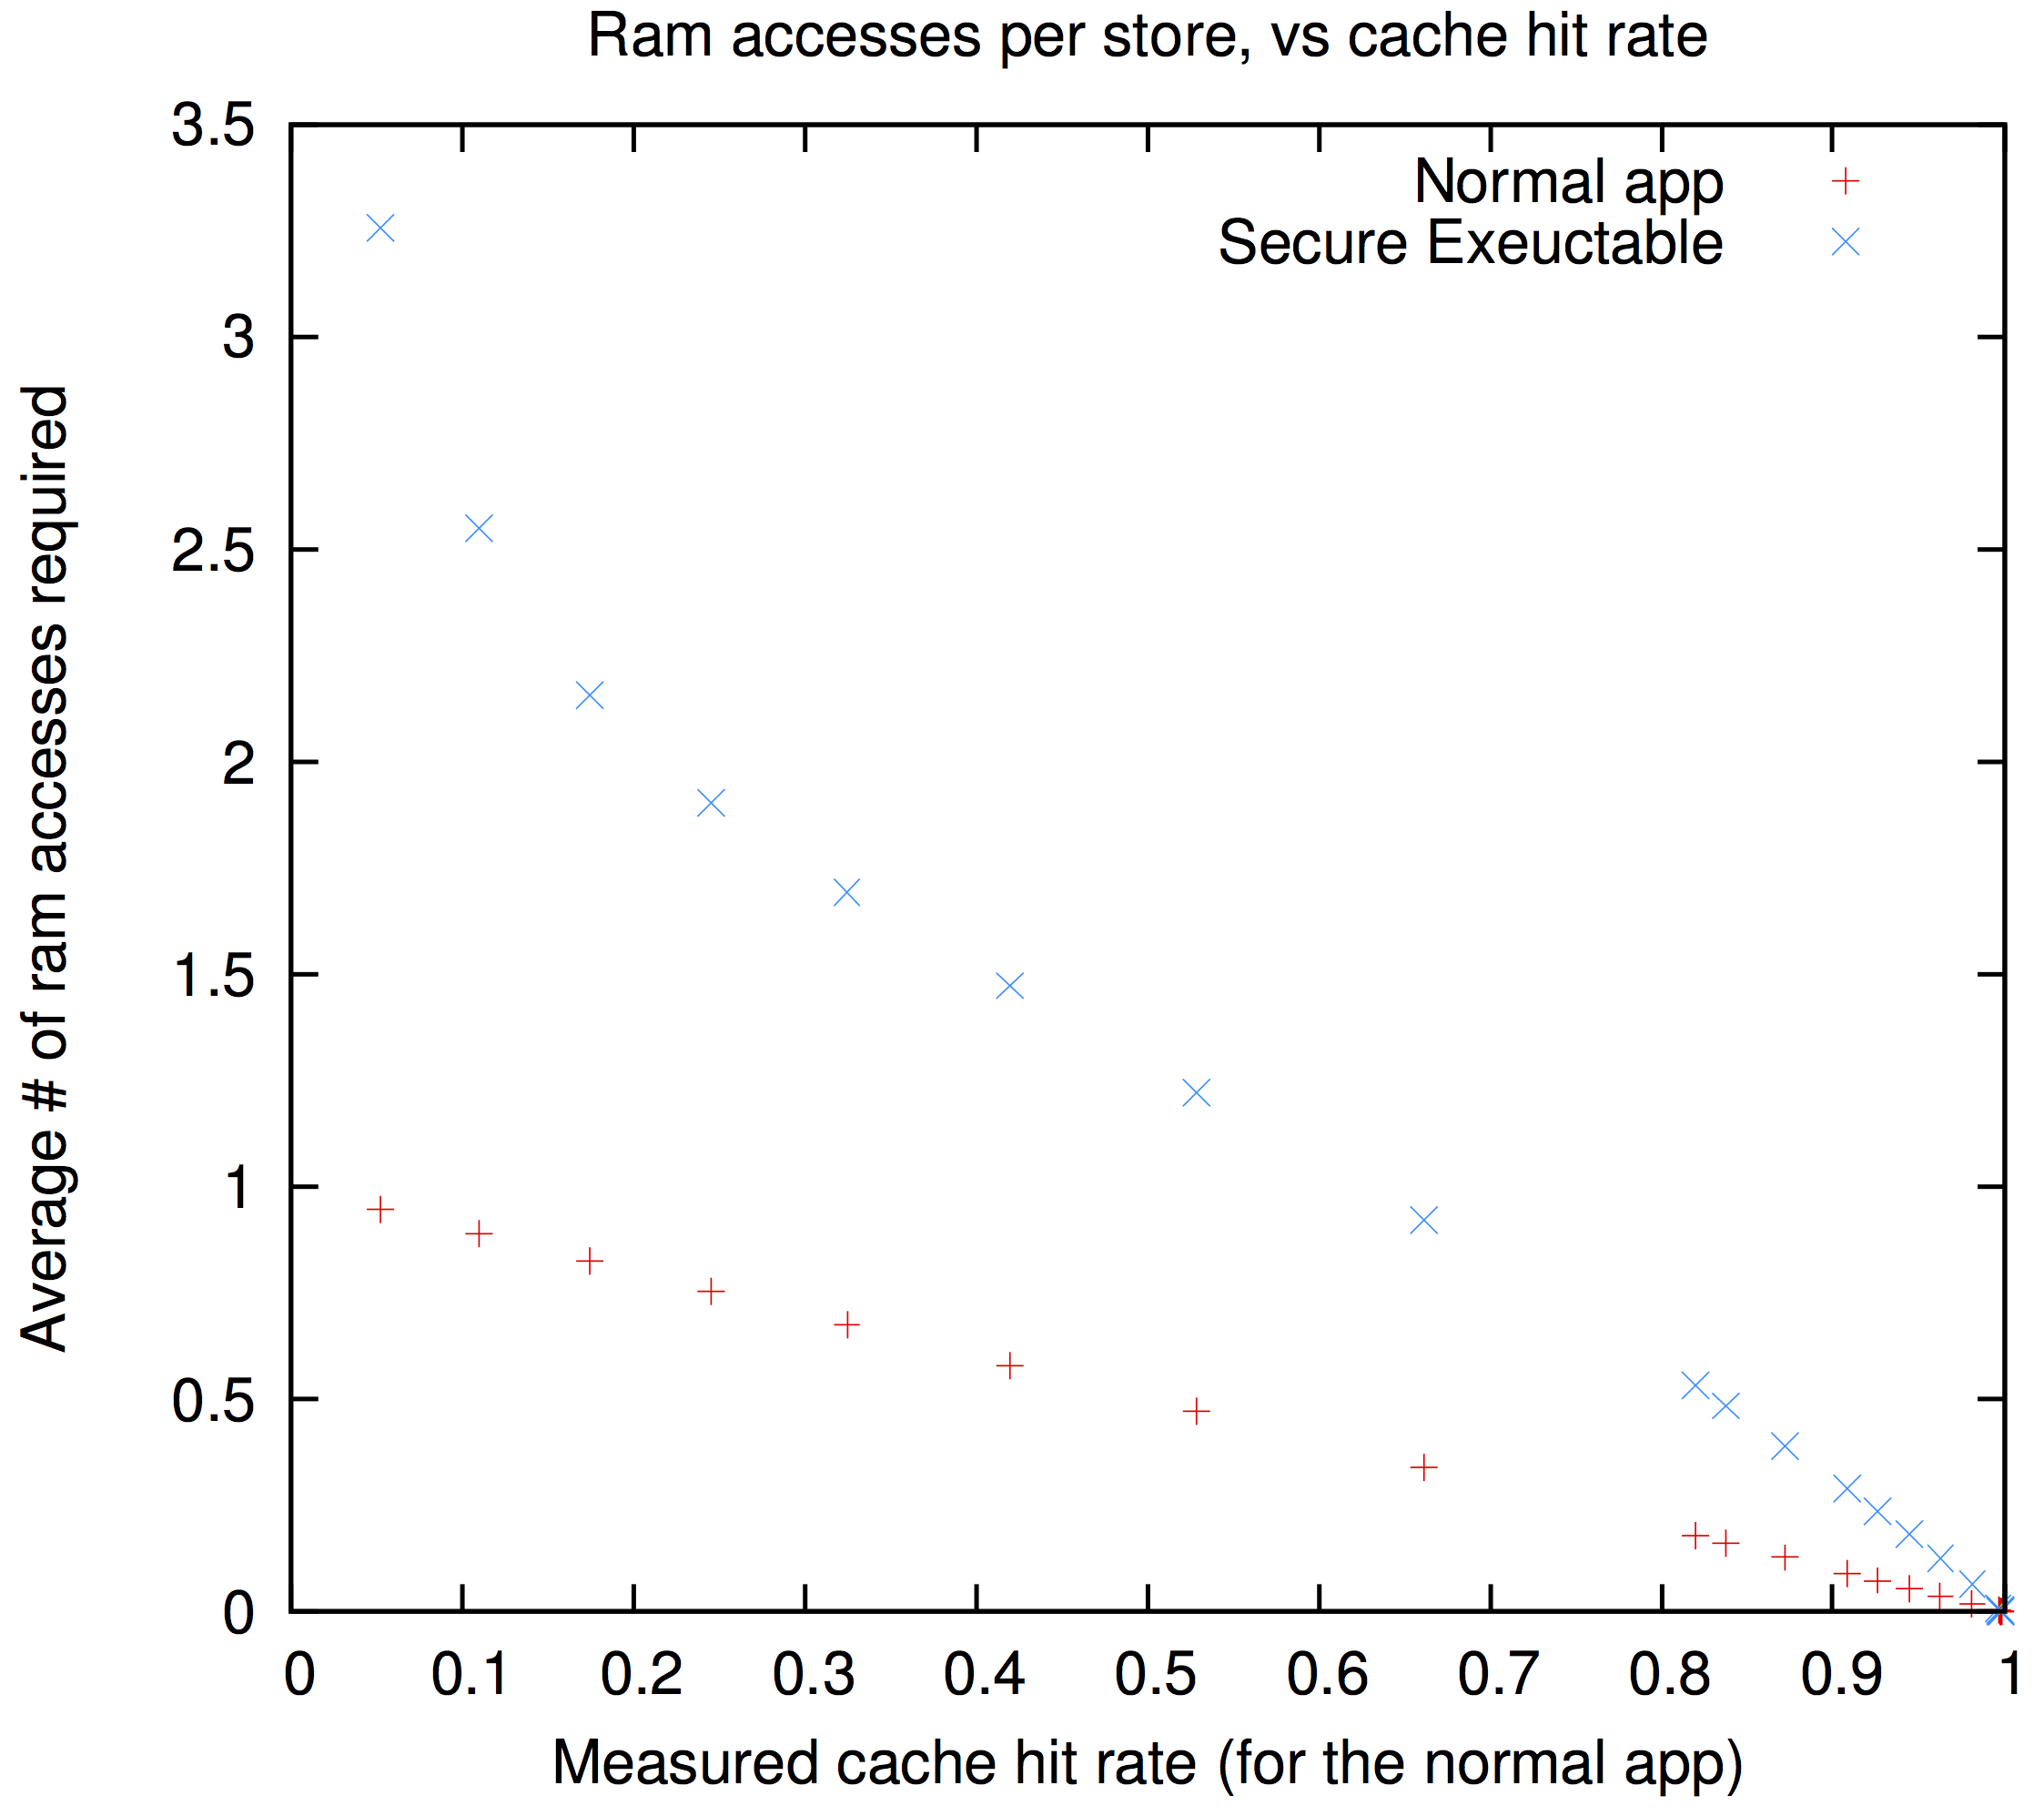
\includegraphics[width=\columnwidth]{bench_per_store2}
		\caption{Schreiben}
		\label{fig:bench_store}
	\end{subfigure}
	\caption{Anzahl der durchschnittlich benötigen RAM-Zugriffe beim lesen / schreiben von Cache Lines\cite{boivie2013secureblue++:big}}
	\label{fig:bench}
\end{figure}

\begin{table}[t]
	\centering
	\small
%	\begin{tabular}{|c*{7}{|p{1.7cm}}|}
%		\hline &
%		Feinheit des Schutzes&
%		OS in der TCB&
%		Limitiert die Anwendung&
%		Hardware\-beschleuni\-gung&
%		Dynamisch wachsender gesicherter Speicher&
%		Anwendung ist Verschlüsselt&
%		Geheimnisse nur im speziellen Bereichen \\
%		\hline
%		SecureBlue++ &
%		\cellcolor{red!25}Prozess &
%		\cellcolor{green!25}N&
%		\cellcolor{green!25}N&
%		\cellcolor{red!25}N&
%		\cellcolor{green!25}J&
%		\cellcolor{yellow!25}J&
%		\cellcolor{green!25}N
%		\\ \hline
%		Intel SGX \cite{mckeen2013innovative}&
%		\cellcolor{green!25}Virtuelle Speicherregion&
%		\cellcolor{green!25}N&
%		\cellcolor{green!25}N&
%		\cellcolor{green!25}J&
%		\cellcolor{red!25}N&
%		\cellcolor{yellow!25}N&
%		\cellcolor{red!25}J\\\hline
%		%\label{tab:vergleich}
%	\end{tabular}
\begin{tabular}{|p{.63\columnwidth}|p{.12\columnwidth}|p{.12\columnwidth}|} \hline
	& SB & SGX \cite{mckeen2013innovative} \\
	\hline 
	
	Feinheit des Schutzes& \cellcolor{red!25}Prozess & \cellcolor{green!25}Virtuelle Speicherregion \\\hline
	OS in der TCB& 	\cellcolor{green!25}N& 	\cellcolor{green!25}N \\\hline
	Limitiert die Anwendung& 	\cellcolor{green!25}N& \cellcolor{green!25}N \\\hline
	RAM Validierung hardwarebeschleunigt & \cellcolor{red!25}N& \cellcolor{green!25}J \\\hline
	Dynamisch wachsender Speicher& \cellcolor{green!25}J & \cellcolor{red!25}N \\\hline
	Anwendung ist Verschlüsselt& \cellcolor{yellow!25}J& \cellcolor{yellow!25}N \\\hline
	Geheimnisse nur im speziellen Bereichen & \cellcolor{green!25}N  & \cellcolor{red!25}J\\\hline
	An die CPU gebunden & \cellcolor{red!25}J  & \cellcolor{green!25}N\\\hline
\end{tabular}
	\caption{Vergleich zwischen SecureBlue++ (SB) und SGX, Grün ist ein Vorteil und Rot eine Limitierung \cite{evtyushkin2014iso}}
\end{table}

Das SecureBlue++ Projekt ist seit 2011 in Entwicklung und es gibt aktuell keine echten POWER CPUs die die SecureBlue++ Erweiterung unterstützen. Deswegen sind alle Benchmarks und Performance-Analysen sehr mit Vorsicht zu genießen und die echten Leistungsdaten können sehr viel schlechter als die simulierten sein.

Für die Benchmark-Simulation wurde eine Anwendung emuliert die auf eine Sequenz von $10^6$ Adressen in einer Exponentialverteilung zugreift. Für den Cache wurde eine Größe von $4096$ Zeilen mit $8$ Spalten und jeweils einer Größe von $32$ Wörtern gewählt. Des weiteren wurden die Ver- und Entschlüsselungen nicht simuliert. Diese würden die Ergebnisse der sicheren Anwendung nochmals in der Reaktionszeit verschlechtern. Hauptsächlich soll mit dem Benchmark gezeigt werden, wie der Integrity Tree aus \cref{sec:Integritätsbaum} die Anzahl der benötigten RAM-Zugriffe für schreibenden bzw. lesenden Zugriff auf die Cache Lines beeinflusst.

Für eine normale Anwendung ist das Lesen von Cache Lines in \cref{fig:bench_load} eine  Gerade, weil bei jedem Cache Miss nur die jeweilige Line mit einem einzigen RAM-Zugriff geladen werden muss. Bei der simulierten gesicherten Anwendung muss für jede zu landende Cache Line auch der jeweilige Knoten des Integrity Tree mit all den Elternknoten geladen werden, da die Cache Lines mit dem Integrity Tree validiert werden. 

Beim Beschreiben von Cache Lines in \cref{fig:bench_store} muss bei einer normalen Anwendung nur die jeweilige Line geändert werden. Sollte diese noch nicht im Cache vorliegen, muss diese mit einem einzigen Zugriff geladen werden. Bei der gesicherten Anwendung muss hierfür ebenfalls wie beim Lesen der jeweilige Knoten des Integrity Trees geladen werden. Des weiteren muss der Baum geändert werden und diese Änderungen werden bis zur Wurzel des Baums durch gedrückt. Deswegen steigen die Anzahl der RAM-Zugriffe sehr viel stärker als beim Lesen an.

\section{Vergleich mit Intel SGX}

Neben SecureBlue++ gibt es auch weitere Ansätze zur isolierten Ausführung von Anwendungen. Am bekanntesten ist Intel SGX \cite{costanintel}, welche mit SecureBlue++ einige Gemeinsamkeiten besitzt. Die größten Unterschiede zwischen beiden Varianten ist, das SecureBlue++ nativ die Verschlüsselung der Anwendung unterstützt und das die gesamte Anwendung in der sicheren Enklave läuft. Bei SGX hingegen kann eine Anwendung aus mehreren Enklaven bestehen und muss nicht für jede CPU einen neuen Schlüssel erhalten.

%\cref{tab:vergleich} 
Tabelle 1. vergleicht SGX mit SecureBlue++. Hierbei bedeutet Grün das es ein Vorteil und Rot ein Nachteil ist. Bei Gelb ist es nicht eindeutig ob es sich um einen Vorteil oder Nachteil handelt. 

\section{Zusammenfassung}
IBMs SecureBlue++ ist in der Theorie eine interessante Befehlssatzerweiterung für die gesicherte und isolierte Ausführung von Anwendungen, die mit den Konkurrenzprodukten anderer Firmen wie Intels SGX mithalten. Leider existiert SecureBlue++ noch nicht als benutz- und evaluierbare Version auf einer realen CPU. Somit sind alle Überlegungen und Vorteile nur theoretischer Natur. Des weiteren existieren versteckte Einschränkungen die den Einsatz in Coud-Computing-Bereich sehr erschweren. 

Der AES-Schlüssel für die Applikation ist mit dem öffentlichen Schlüssel von einer CPU verschlüsselt. Somit kann die Anwendung auch nur auf dieser einen CPU ausgeführt werden. Jedoch hat man im Coud-Computing-Bereich meist keinen direkten Einfluss auf welcher physischen Maschine die Anwendung ausgeführt wird. 

Viele wichtige Informationen wie zum Beispiel die Limitierung der \emph{SET} oder auf welchen Komponenten die \emph{PMT} oder \emph{MRMT} gespeichert werden fehlen aktuell. 

Durch die Verschlüsselung der Anwendung wäre es theoretisch möglich auf einem kompromittierten System eine gesicherte Anwendung als Malware auszuführen ohne das der Betreiber des Rechenzentrums analysieren kann was diese Anwendung macht \cite{davenport2014sgx}.

In den kommenden POWER9 CPUs sollen erste Versionen von SecureBlue++ zur Verfügung stehen und dann wird sich zeigen, ob SecureBlue++ die aufgestellten Erwartungen erfüllen kann.

\small
\bibliographystyle{abbrv}
\bibliography{sigproc}  
\end{document}
